\documentclass{VUMIFPSkursinis}
\usepackage{algorithmicx}
\usepackage{algorithm}
\usepackage{algpseudocode}
\usepackage{amsfonts}
\usepackage{amsmath}
\usepackage{bm}
\usepackage{caption}
\usepackage{color}
\usepackage{float}
\usepackage{graphicx}
\usepackage{listings}
\usepackage{subfig}
\usepackage{wrapfig}
\usepackage{multirow}
\usepackage{longtable}
\usepackage{array,makecell}

% Titulinio aprašas
\university{Vilniaus universitetas}
\faculty{Matematikos ir informatikos fakultetas}
\department{Programų sistemų katedra}
\papertype{Programų sistemų inžinerija}
\title{Stalo žaidimų programėlė}
\titleineng{BOARD GAMES APPLICATION}
\status{2 kurso 5 grupės studentai}
\author{Elena Reivytytė}
\secondauthor{Matas Šilinskas}
\thirdauthor{Kasparas Taminskas}
\fourthauthor{Aidas Vaikšnoras}
\fifthauthor{Tadas Žaliauskas}
\supervisor{dr. Vytautas Valaitis}
\date{Vilnius – \the\year}

% Nustatymai
% \setmainfont{Palemonas}   % Pakeisti teksto šriftą į Palemonas (turi būti įdiegtas sistemoje)
\bibliography{bibliografija}

\begin{document}
\maketitle

\sectionnonum{Anotacija}
Šis dokumentas yra trijų Programų sistemų inžinerijos kurso laboratorinių darbų rezultatas, aprašantis
mobiliosios stalo žaidimų programėlės projekto kūrimo procesą, todėl jo turinys išskaidytas į šias dalis:

Pirmosios dalies, 3-iojo laboratorinio darbo, rezultato - paruošto dokumento  - turinys susideda iš išsamaus dalykinės srities verslo proceso tyrimo, kurį sudaro vidinė ir išorinė verslo procesų analizė, jų rezultatas - SSGG diagrama,  galimos problemos ir jų sprendimo būdai, verslo modelį (sistemos panaudojimą) atspindinčios aukšto lygmens UML diagramos, taip pat sistemos įgyvendinamumo analizė, parodanti realias galimybes įeiti į rinką. Programėlės tikslas yra suvienyti žmones, esančius artimoje aplinkoje ir mėgstančius žaisti stalo žaidimus, taip būtų sukuriamas specializuotas stalo žaidimų fanų socialinis tinklas. Mobiliosios programėles tikslinė auditorija yra žmonės, mėgstantys stalo žaidimus, esantys tam tikrose uždarose grupėse (pvz. butų, bendrabučių gyventojai ar festivalių dalyviai) ieškantys žaidėjų stalo žaidimams. 

Antrosios dalies turinys yra skirtas aprašyti stalo žaidimų mobiliosios programėlės reikalavimų specifikacijai. Dokumente išdėstomi pagrindiniai sistemos reikalavimai, kurie formuluojami po dalykinės verslo srities analizės jau turint konkretesnį kuriamos sistemos poreikių sąrašą.

Paskutinėje dokumento dalyje pristatomas mobiliosios stalo žaidimų programėlės Board Games 4+1 architektūrinis modelis, kurį sudaro loginis, kūrimo, fizinis, procesų ir užduočių pjūviai, visi kartu parodantys sistemą iš skirtingų pusių, papildantys vieni kitus. Modelio pagrindas - standartinės UML diagramos.

\tableofcontents

\sectionnonum{Žodynas}
\begin{enumerate}
\item Aplikacija - tai programėlė leidžianti naudotis aprašytomis funkcijomis.
\item Naudotojas - tai bendrinis aplikacijos profilis.
\item Žaidimas - stalo žaidimo įvykis. (Game)
\item Vartotojas - galutinis aplikacijos vartotojas, galintis sukurti ar prisijungti prie egzistuojančio žaidimo. (User)
\item Administratorius - tai žmogus kuris prižiūri korektišką aplikacijos veikimą, turi priėjimą prie statistinės informacijos.
\item Kompanija - verslo subjektas, galintis aplikacijoje sukurti specialus renginius savo atstovaujamiems žaidimams.
\item Draugas - tai vartotojas esantis draugų saraše, kuriam galima parašyti žinutę arba pakviesti žaisti konkretų žaidimą. (Friend)
\item Perspektyva - (Point of view) aplikacijos naudojimo kampas priklausantis nuo naudotojo tipo.

\end{enumerate} 

\section{Verslo srities analizė}

\subsection{Įvadas}
\textbf{Darbo tikslas}\\
Išanalizuoti esamą stalo žaidimų organizavimo rinką ir pasitelkus dalykinės srities verslo procesų analizę sukurti naują projektą, 
gebantį sujungti žmones bendram laisvalaikio praleidimui žaidžiant stalo žaidimus, pasitelkiant 
inovatyvias idėjas ir pateikti sprendimą, pagelbėsiantį trūkstamų žaidimo draugų paieškoje.

\textbf{Temos aktualumas}\\
Stalo žaidimai, kaip alternatyva kompiuteriniams žaidimams, išlaiko gausų gerbėjų ratą - tai 
yra žmones, kurie vertina gyvą bendravimą. Be to ši žaidėjų auditorija yra itin tikslinė ir 
lojali. Bendrabučiuose ir festivaliuose žmonės dažnai buriasi į grupeles smagiai praleisti 
laisvalaikį prie žaidimų lentos. Iki šiol stalo žaidimų organizavimu vertėsi tik specializuotos 
kavinės, tačiau tokių kavinių mastas yra mažas, o žaidimai vykdavo gana retai, organizatorių 
nustatytoje vietoje, tad reikėdavo papildomai keliauti iš namų. Tačiau iškyla problema, kaip, 
žaidimui pritrūkus žmonių, visiškai nepažįstami žmonės irgi galėtų būti įtraukti į tokį laisvalaikio 
praleidimo būdą. Į pagalbą ateitų mūsų programėlė, kuri leistų atrasti planuojamus žaisti stalo 
žaidimus aplink ir prie jų prisijungti pateikus prašymą.

\textbf{Siekiami rezultatai}\\
Mes siekiame padidinti žmonių susidomėjimą stalo žaidimais, skatiname juos rinktis tokią veiklą 
ir sukurti stalo žaidimus apjungiančią sistemą. Tikimasi, kad mėgėjai aktyviai kurs ir kvies 
kitus prisijungti prie stalo žaidimų, o nerandantys su kuo žaisti, atras sau žaidimo draugų. 
Siekiame, kad programėlė pritrauktų ir žaidimų platintojus plačiai reklamuotis programėlėje, 
kurie siūlytų išbandyti naujus, didelio susidomėjimo sulaukusius žaidimus už teikiamą paramą mums.

\subsection{Verslo proceso aprašymas}
Nagrinėjama verslo sritis - stalo žaidimai. Jie dažniausiai žaidžiami ant žaidimo 
lentos ar kitaip pažymėto žaidimo ploto su specialiais žaidimo komponentais 
(kauliukai, figūrėlės, kortelės).

\textbf{Nagrinėjamos srities apibrėžimas:}\\
Stalo žaidimai, įdomus ir linksmas laisvalaikio praleidimo būdas, aktyvus 
laisvalaikis, pramogos

\textbf{Dalykinė sritis:}\\
Stalo žaidimai ir pagalba juos organizuojant

\textbf{Probleminė sritis:}\\
Plataus spektro stalo žaidimų organizavimas, yra žaidėjų, kurie organizuoja 
žaidimą, tačiau jiems trūksta žaidėjų, kad žaidimas įvyktų, taip pat yra žmonių, 
kurie nori žaisti konkretų žaidimą, bet neturi draugų, norinčių žaisti tą žaidimą.

Daugeliui, išgirdus žodį „stalo žaidimai“, galvoje sukuriama asociacija 
su vaikais ar paaugliais. Tačiau stalo žaidimų yra labai daug ir įvairių, 
sukurtų skirtingoms amžiaus grupėms, reikalaujančių skirtingų žaidėjo savybių 
(strateginis mąstymas, diplomatiniai sugebėjimai, rankų miklumas, kūrybiniai 
gebėjimai) ir naudojančių skirtingus žaidimo komponentus. Dauguma net nesusimąsto, 
kad stalo žaidimai turi ir mokomąja vertę. Tarp gausybės spalvingų žaidimų galima 
rasti tokių, kurie vysto vaiko raidą, padeda pažinti raides ir mokytis skaityti, 
lavina matematinius, loginius bei kūrybinius įgūdžius. Vis dažniau prie stalo 
žaidimų galima sutikti ir vyresnių, net ir garbaus amžiaus žmonių, susižavėjusių 
šia turininga ir užkrečiančia pramoga, kuri tampa lyg šeimos tradicija susirinkti 
prie bendro stalo. Neretai kalbant apie stalo žaidimus omenyje taip pat turimi ir 
klasikiniai žaidimai (šachmatai, šaškės, domino), kortų žaidimai ar vaidmenų žaidimai.\\
Ilgą laiką beveik išimtinai aukštuomenės pramoga buvę stalo žaidimai, kaip idealus 
šeimos laisvalaikio leidimo būdas, išpopuliarėjo JAV XX amžiaus viduryje. 
Didžiausias pagyvėjimas po vėliau prarastų pozicijų kompiuteriniams ir konsolių 
žaidimams, „gyvų“ žaidimų rinkoje buvo juntamas 9-ajame dešimtmetyje, atsiradus 
kolekcionuojamiems kortų žaidimams ir padidėjus modernių stalo žaidimų populiarumui.\\
Savo mobiliąja programėle stengsimės padidinti stalo žaidimų populiarumą suteikiant 
geresnes sąlygas siekiant surasti trūkstamų žaidėjų skaičių, kitaip tariant 
supaprastinant žaidimo organizavimo procesą, kuris be tokios platformos yra gana 
keblus, nes žaidimui reikia neretai 4-10 žaidėjų, kurie būtų pasiruošė paskirti 
pora valandų žaidimo sesijai.

\subsection{Išorinė proceso analizė}
	\subsubsection{Dabartinio verslo sistemos įeiga:}
		\renewcommand{\labelitemi}{$\bullet$}
			\begin{itemize}
				\item Žaidėjo registracijos duomenys. Ši įeiga pasirinkta todėl, 
				kad ji yra būtina šiuolaikiniame versle. Žaidėjai, neįvedę 
				registracijos duomenų - vardo, pavardės, prisijungimo vardo, 
				elektroninio pašto - negali naudotis programėle. Dėl saugumo tikslų 
				taip pat galima pateikti nuotrauką taip parodant, kad naudotojas 
				nebijo atskleisti savo tapatybės kitiems žaidėjams.
				\item Rėmėjai (stalo žaidimų prekyba užsiimantys verslai).
				\item Žaidėjai, kuriantys žaidimų sesijas.
				\item Stalo žaidimų klubai (pvz. RIKIS).
			\end{itemize}
	\subsubsection{Dabartinio verslo sistemos išeiga:}
		\renewcommand{\labelitemi}{$\bullet$}
			\begin{itemize}
				\item Žaidimo, laukimo laikas ir atstumas iki žaidimo vietos. 
				Šios charakteristikos pasirinktos tam, kad vartotojas galėtų 
				nustatyti, ar verta prisijungti ir dalyvauti žaidime. Vartotojas 
				gali pasirinkti nedalyvauti žaidime, kuris yra toli nuo jo namų 
				arba jo žaidimo/ laukimo iki pradžios laikas yra per didelis.
				\item Sėkmingai įvykę stalo žaidimų susibūrimai.
				\item Prizai, skatinantys dalyvių aktyvumą.
				\item Žaidėjų atsiliepimai, palikti po įvykusio stalo žaidimo.
			\end{itemize}
	\subsubsection{Dabartinis verslas reguliuojamas šių taisyklių:}
		\renewcommand{\labelitemi}{$\bullet$}
			\begin{itemize}
				\item Viešai atskleisti trečiosioms šalims ar naudoti pateiktus 
				vartotojo duomenis be jo sutikimo yra draudžiama.
				\item Ribotas kapitalo kiekis veiklos pradžioje.
			\end{itemize}
	\subsubsection{Dabartinis verslo įvaizdžio formavimas:}
		\renewcommand{\labelitemi}{$\bullet$}
			\begin{itemize}
				\item Atsiliepimai internete,
				\item Reklama socialiniuose tinkluose.
				\item Rėmėjų steigiami prizai.
				\item Remėjų rengiami konkursai ir varžybos.
			\end{itemize}
			
	\subsubsection{Įeigos metrikos}			
		\begin{longtable}{ | m{3.5cm} | m{3.5cm} | m{3.5cm} | >{\centering}m{1.6cm} | >{\centering}m{1.6cm} | }
		\caption{Įeigos metrikos}
		\label{variability_impl_mech}
		%\endfirsthead
		\endhead
		 \hline			

		\centering{\textbf{Metrika}} & \centering{\textbf{Matavimo vienetas}} & \textbf{Kaip matuoti} & \textbf{Dabartinė reikšmė} & \textbf{Kritinė reikšmė} \tabularnewline \hline
		Žaidėjo registracijos duomenys. & Procentas žaidėjų, kurie pateikė vardą. & Suskaičiuoti dalį žaidėjų, kurie pateikė vardą. & 100\% & 100\% \tabularnewline \hline
		Žaidėjo registracijos duomenys. & Procentas žaidėjų, kurie pateikė pavardę. & Suskaičiuoti dalį žaidėjų, kurie pateikė pavardę. & 100\% & 100\% \tabularnewline \hline
		Žaidėjo registracijos duomenys. & Procentas žaidėjų, kurie pateikė prisijungimo vardą. & Suskaičiuoti dalį žaidėjų, kurie pateikė prisijungimo vardą. & 100\% & 100\% \tabularnewline \hline
		Žaidėjo registracijos duomenys. & Procentas žaidėjų, kurie pateikė elektroninį paštą. & Suskaičiuoti dalį žaidėjų, kurie pateikė elektroninį paštą. & 100\% & 100\% \tabularnewline \hline
		Žaidėjo registracijos duomenys. & Procentas žaidėjų, kurie pateikė nuotrauką. & Suskaičiuoti dalį žaidėjų, kurie pateikė nuotrauką. & 50\% & 50\% \tabularnewline \hline
		Atstumas nuo žaidėjo iki žaidimo vietos. & Vidutinis nukeliaujamas atstumas nuo žaidėjo iki žaidimo vietos. & Suskaičiuoti visų žaidėjų, išskyrus žaidimo kūrėjų, kiekvieno žaidimo nuvyktą atstumą ir išvesti vidurkį. & 0.8 km & 1.0 km \tabularnewline \hline
		Žaidimo trukmė. & Vidutinė žaidimo trukmė valandomis. & Suskaičiuoti vykusių žaidimų trukmes ir išvesti vidurkį. & 3.5 h & 4.0 h \tabularnewline \hline
		Laukimo trukmė. & Vidutinė laukimo iki žaidimo pradžios trukmė valandomis. & Suskaičiuoti laukimo iki žaidimų pradžių trukmes ir išvesti vidurkį. & 1.5 h & 1.0 h \tabularnewline \hline
		Vartotojo pateikiamas mokestis už žaidimo iškėlimą. & Procentas vartotojų, kurie pirko paslaugą. & Suskaičiuoti, dalį vartotojų, kurie naudojosi mokama paslauga iškelti žaidimą visų sąraše, o kiek nemokama. & Mokama: 1\% Nemokama: 99\% & Mokama: 5 \% Nemokama: 95 \% \tabularnewline \hline
		Žaidimų duomenys. & Visų įvykusių žaidimų skaičius. & Suskaičiuoti visų įvykusių žaidimų skaičių. & 60\% & 80\% \tabularnewline \hline
		Žaidimų duomenys. & Visų neįvykusių žaidimų skaičius. & Suskaičiuoti visų neįvykusių žaidimų skaičių. & 40\% & 20\% \tabularnewline \hline
		Žaidimų duomenys. & Vidutinis žmonių kiekis žaidime. & Suskaičiuoti visų įvykusių žaidimų žaidėjų skaičių ir išvesti vidurkį. & 6 & 6 \tabularnewline \hline
		Žaidimų duomenys. & Aktyvių programėlės naudotojų, dalyvaujančių žaidimuose, skaičius. & Suskaičiuoti žaidėjus, kurie per savaitę sužaidžia bent vieną žaidimą. & 0 & 1000 \tabularnewline \hline
		Žaidimų duomenys. & Vidutinis asmeninių išsiųstų žinučių kiekis per mėnesį. & Suskaičiuoti visų asmeninių išsiųstų žaidėjų žinutes ir išvesti vidurkį. & 75 & 100 \tabularnewline \hline
		Žaidimų duomenys. & Vidutinis išsiųstų žinučių kiekis žaidimo kūrimo lange per mėnesį. & Suskaičiuoti visų išsiųstų žaidėjų žinutes žaidimo kūrimo lange ir išvesti vidurkį. & 325 & 500 \tabularnewline \hline
		Rėmėjų duomenys. & Rėmėjų, užsiimančių žaidimų prekyba ir norinčių remti programėlę mainais už reklamą, skaičius. & Suskaičiuoti visus rėmėjus, užsiimančius žaidimų prekyba ir norinčius remti programėlę mainais už reklamą. & 0 & 7 \tabularnewline \hline
		Rėmėjų duomenys. & Remėjų, užsiregistravusių programėlėje ir reklamuojančių savo prekes, sukurtų prekės pristatymo renginių vidurkis. & Suskaičiuoti, kiek renginių kiekviena kompanija inicijuoja ir išvesti vidurkį. & 0 & <5 \tabularnewline \hline
		Rėmėjų duomenys. & Vidutinis skaičius žaidėjų, sekančių užsiregistravusį remėją. & Suskaičiuoti, kiek žaidėjų seka kiekvieną užsiregistravusį remėją ir išvesti vidurkį. & 0 & <5 \tabularnewline \hline
	    \end{longtable}
		
	\subsubsection{Išeigos metrikos}			
		\begin{longtable}{ | m{3.5cm} | m{3.5cm} | m{3.5cm} | >{\centering}m{1.6cm} | >{\centering}m{1.6cm} | }
		\caption{Įeigos metrikos}
		\label{variability_impl_mech}
		%\endfirsthead
		\endhead
		 \hline			

		\centering{\textbf{Metrika}} & \centering{\textbf{Matavimo vienetas}} & \textbf{Kaip matuoti} & \textbf{Dabartinė reikšmė} & \textbf{Kritinė reikšmė} \tabularnewline \hline
		Kasdienių suorganizuotų žaidimų duomenys. & Procentas žaidėjų, kurie pateikė vardą. & Suskaičiuoti visų žaidimų, sukuriamų per savaitę, skaičių ir išvesti vidurkį. & 0 & 50 \tabularnewline \hline
		Prizai. & Žaidimo monetos, skiriamos prisijungus kiekvieną dieną. & Suskaičiuoti vidutinį monetų skaičių per dieną, kai prisijungiama 7 kartus iš eilės. & 0 & 30 vnt \tabularnewline \hline
		Teigiami žmonių atsiliepimai. & Vidutinis teigiamų atsiliepimų,kuriuos palieka žaidėjai, dalyvavę žaidime, skaičiusi. & Teigiamų žmonių atsiliepimų dalis procentais.a - teigiamų atsiliepimų skaičius, n - bendras atsiliepimų skaičius.  & 50\% & 70\% \tabularnewline \hline
	    Neigiami žmonių atsiliepimai. & Vidutinis neigiamų atsiliepimų, kuriuos palieka žaidėjai, dalyvavę žaidime, skaičius. & Neigiamų žmonių atsiliepimų dalis procentais.a - neigiamų atsiliepimų skaičius, n - bendras atsiliepimų skaičius.  & 30\% & 20\% \tabularnewline \hline
		Reklamos. & Vidutinis skaičius žaidimų, kuriuos reklamuoja kiekvienas rėmėjas. & Suskaičiuoti, kiek žaidimų kiekvienas rėmėjas reklamuoja ir išvesti vidurkį.  & 0 & 7 \tabularnewline \hline
		Teigiamas rėmėjo vertinimas. & Žaidėjų, teigiamai įvertinusių rėmėjo siūlomą žaidimą, kiekis. & Suskaičiuoti, kiek procentaliai žaidėjų teigiamai vertina kompanijos reklamuojamą žaidimą. & 70\% & 20\% \tabularnewline \hline
		Neigiamas rėmėjo vertinimas. & Žaidėjų, neigiamai įvertinusių rėmėjo siūlomą žaidimą, kiekis. & Suskaičiuoti, kiek procentaliai žaidėjų neigiamai vertina kompanijos reklamuojamą žaidimą. & 30\% & 50\% \tabularnewline \hline	
		\end{longtable}
		
\subsection{Vidinė proceso analizė}
	\subsubsection{Verslo proceso tobulinimo strategija}
		\textbf{Vizija:}\\
		Stalo žaidimai yra įdomus, linksmas ir žmones suvienijantis laiko praleidimo 
		būdas, šios veiklos populiarumas pastebimai auga, į žaidimus įsitraukia vis 
		daugiau įvairesnių socialinių grupių atstovų, sukuriamas atskiras specializuotas 
		socialinis tinklas, skirtas stalo žaidimų mėgėjams.

		\textbf{Misija:}\\
		Sukurti mobiliąją aplikaciją, kuria naudojantis žmonės lengvai galėtų 
		surasti trūkstamų žaidėjų stalo žaidimams ir užmegzti naujas pažintis su 
		jais arba sustiprinti esamas

		\textbf{Tikslai:}\\
		Pagrindinis tikslas yra sukurti gerą sistemos prieinamumą sukuriant 
		mobiliąją programėlę stalo žaidimams, kuri palengvina žaidimų organizavimą.

		\subsubsubsection{Bendroji tobulinimo strategija:}
			\textbf{Organizacinio proceso supaprastinimas}
			\renewcommand{\labelitemi}{$\bullet$}
				\begin{itemize}
					\item Palengvinti stalo žaidimų organizatorių darbą ir apmažinti organizacinės veiklos kiekį.
					\item Suteikti galimybę žaidėjams žaisti nemokamai, laisvai pasirinkti norimą stalo žaidimų vietą ir patogų laiką, pvz. nepriklausomai nuo stalo žaidimų klubų siūlomų vietos ir laiko bei renkamo dalyvio mokesčio.
					\item Pagerinti galutinio produkto reklamos metodiką ir informacijos platinimą, kad žinios apie jį pasiektų visuomenę ir į laisvalaikio praleidimą žaidžiant stalo žaidimus įsitrauktų kuo daugiau žmonių.
				\end{itemize}	

			\textbf{Pagerintas sistemos prieinamumas}
			\renewcommand{\labelitemi}{$\bullet$}
				\begin{itemize}
					\item Išsirinkti norimą/-as mobiliasias platformas, kuriose bus palaikoma programėlė.
					\item Sugalvoti, kokius funkcionalumus palaikys mobilioji programėlė.
					\item Suprogramuoti aplikaciją.
					\item Patobulinta grafinė vartotojo sąsaja.
				\end{itemize}	

		\subsubsubsection{Struktūrizuota tobulinimo strategija}
			\textbf{Organizacinio proceso supaprastinimas}\\
			Panaudoti programėlę siekiant:
			\renewcommand{\labelitemi}{$\bullet$}
				\begin{itemize}
					\item Pasiekti visus susidomėjusius stalo žaidimais netoliese.
					\item Supaprastinti pažinčių mezgimo procesą (networking).
					\item Palengvinti žaidimui prasidėti reikalingų trūkstamų žmonių paiešką.
					\item Patalpinti visus vykstančius stalo žaidimus į vieną vietą, kad vartotojai centralizuotoje platformoje patogiai galėtų rinktis prie kokio žaidimo prisijungti.
					\item Nesunkiai suderinti žaidimo laiką ir vietą, patogią visiems užsiregistravusiems žaidėjams.
				\end{itemize}	

			\textbf{Programėlės populiarinimas}
			\renewcommand{\labelitemi}{$\bullet$}
				\begin{itemize}
					\item Kvietimai išbandyti programėlę, skelbiami socialiniuose tinkluose.
					\item Skrajutės bendrabučiuose, festivaliuose, specializuotose stalo žaidimų parduotuvėse.
					\item Naujienlaiškiai į elektroninį paštą.
					\item Įsteigti prizus aktyviausiems žaidimų kūrėjams, taip didinant žmonių susidomėjimą naudotis programėle.
					\item Rengiant varžybas, konferencijas, turnyrus.
					\item Rengiant internetines laidas apie naujausius įvykius stalo žaidimų pasaulyje.
					\item Rengiant tiesiogines transiliacijas Twitch, facebook, youtube platformose.
					\item Aktyviai skelbiamas turinys twitter, facebook, instagram, snapchat socialiniuose tinkluose.
				\end{itemize}
				
			\textbf{Geras sistemos prieinamumas}
			Sukurti mobiliąją aplikaciją stalo žaidimams. Įgyvendinimo žingsniai:
			\renewcommand{\labelitemi}{$\bullet$}
				\begin{itemize}
					\item Pasirinkti mobiliasias platformas, kuriose veiks aplikacija.
					\item Sugalvoti funkcionalumus, kuriuos atliks aplikacija.
					\item Sugalvoti patogų ir patrauklų aplikacijos dizainą.
					\item Suprogramuoti aplikaciją.
					\item Surasti patikimą serverių nuomos paslaugų tiekėją..
					\item Suprojektuoti web aplikaciją, turinčią analogišką funkcionalumą kaip ir mobiliosios aplikacijos.
				\end{itemize}
				
	\subsubsection{Esamų sistemų analizė}
		\subsubsubsection{Rikis – stalo žaidimų klubas}
			\textbf{Sistemos veikimas}\\
			Klubas apie savo veiklą skelbia facebook socialiniame tinkle, prieš 
			organizuodamas žaidimų vakarą, sukuria įvykį ir juo pasidalina. 
			Dalyvavimas yra nemokamas klubo nariams, visiems kitiems yra taikomas 
			simbolinis 1 EUR „kėdės“ mokestis. Laukiami tiek patyrę, tiek nauji 
			stalo žaidimų entuziastai. Stalo žaidimai žaidžiami toje pačioje vietoje 
			– RIKIO stalo žaidimų parduotuvėje.

			\textbf{Sistemos trūkumai ir kylančios problemos:}\\
			Organizacija turi pastovų žaidėjų ratą, kuriam plėstis sunku dėl to, 
			nes kai kuriems žaidėjams nekintanti žaidimo vieta gali būti neparanki 
			(tolimas atstumas nuo namų). Žaidimai vyksta nustatytu laiku, kuris 
			neretai yra nepatogus ir prie jo tenka prisiderinti. Ribotas žaidimų 
			pasirinkimas, nes žaidžiama su tuo, ką parduotuvė gali pasiūlyti. 
			Dalyvavimas yra mokamas, o vietų skaičius ribotas.
				
		\subsubsubsection{Board Gamer programėlė}
			\textbf{Sistemos veikimas}\\
			Klubas apie savo veiklą skelbia facebook socialiniame tinkle, prieš 
			organizuodamas žaidimų vakarą, sukuria įvykį ir juo pasidalina. 
			Dalyvavimas yra nemokamas klubo nariams, visiems kitiems yra taikomas 
			simbolinis 1 EUR „kėdės“ mokestis. Laukiami tiek patyrę, tiek nauji 
			stalo žaidimų entuziastai. Stalo žaidimai žaidžiami toje pačioje vietoje 
			– RIKIO stalo žaidimų parduotuvėje.
			
			\textbf{Sistemos trūkumai ir kylančios problemos:}\\
			Dauguma sistemos naudotojų komentaruose skundžiasi, kad programėle 
			naudojasi per mažai žmonių, tad susitarti dėl žaidimo tampa labai sunku. 
			Tai gali signalizuoti apie mažą dalykinės srities aktualumą žmonėms arba
			prastai įvykdytą programėlės reklamos kampaniją. Kitas gana svarbus 
			trūkumas yra, kad programėlė, įvedus į paiešką jos pavadinimą, sąraše 
			rikiuojasi tik dvidešimtoje pozicijoje, todėl net ir žinantiems, ko 
			ieško, vartotojams tampa ypatingai keblu programėlę surasti dėl ne itin 
			unikalaus jos pavadinimo. Gana didelis trūkumas yra kitų mobiliųjų 
			platformų palaikymo nebuvimas, nes programėlė prieinama tik iOS įrenginiams.

		\subsubsection{Analizės rezultatai}
			Stiprybės, silpnybės, galimybės ir grėsmės.		
			\begin{longtable}{ | m{8cm} | m{8cm} | }
			\caption{SWOT}
			\label{variability_impl_mech}
			%\endfirsthead
			\endhead
			 \hline			

			\centering{\textbf{Stiprybės}} & \centering{\textbf{Silpnybės}} \tabularnewline \hline
				\begin{enumerate}
					\item Programėlė žinoma tarp studentų ir mėgstančių stalo žaidimus žmonių, tai užtikrina, kad tose grupėse programėlės populiarumas nemažės.
					\item Programėlė skatina gyvą bendravimą tarp žmonių, ko šiais laikais labai trūksta. Ši programėlė skatina žmones susitikti, praleisti laiką kartu ir taip išsiskiria iš kitų panašaus tipo programėlių, šiuo metu esančių rinkoje.
					\item Programėlės sritis siaura, todėl lengva palaikyti ir atnaujinti sistemą.
					\item Programėlė unikali, tokių rinkoje labai mažai arba nėra, taigi, turėsime labai nedaug konkurentų, galinčių užimti programėlės vietą rinkoje, šis aspektas taip pat užtikrina programėlės populiarumo pastovumą.
				\end{enumerate}
					& 
				\begin{enumerate}
					\item Norint dalyvauti žaidime, reikia pateikti daug asmeninės informacijos, tačiau būtent tai užtikrins mūsų vartotojų saugumą.
					\item Tikėtina, kad programėlė labiausiai bus naudojama vakarais, savaitgaliais ir jos apkrovimas tada bus didelis, kitais paros ir savaitės laikais ji susilauks mažai naudotojų.
					\item Programėlės sėkmė stipriai priklauso nuo naudotojų kiekio - jei jų trūksta, gali tekti ilgai laukti iki žaidimo pradžios. 
					\item Komanda jauna, todėl turi nedaug patirties kuriant kompleksines platformas.
				\end{enumerate}\tabularnewline \hline
			\centering{\textbf{Galimybės}} & \centering{\textbf{Grėsmės}} \tabularnewline \hline
				\begin{enumerate}
					\item Programėlė žinoma tarp studentų ir mėgstančių stalo žaidimus žmonių, tai užtikrina, kad tose grupėse programėlės populiarumas nemažės.
					\item Programėlė skatina gyvą bendravimą tarp žmonių, ko šiais laikais labai trūksta. Ši programėlė skatina žmones susitikti, praleisti laiką kartu ir taip išsiskiria iš kitų panašaus tipo programėlių, šiuo metu esančių rinkoje.
					\item Programėlės sritis siaura, todėl lengva palaikyti ir atnaujinti sistemą.
					\item Programėlė unikali, tokių rinkoje labai mažai arba nėra, taigi, turėsime labai nedaug konkurentų, galinčių užimti programėlės vietą rinkoje, šis aspektas taip pat užtikrina programėlės populiarumo pastovumą.
				\end{enumerate}
					& 
				\begin{enumerate}
					\item Norint dalyvauti žaidime, reikia pateikti daug asmeninės informacijos, tačiau būtent tai užtikrins mūsų vartotojų saugumą.
					\item Tikėtina, kad programėlė labiausiai bus naudojama vakarais, savaitgaliais ir jos apkrovimas tada bus didelis, kitais paros ir savaitės laikais ji susilauks mažai naudotojų.
					\item Programėlės sėkmė stipriai priklauso nuo naudotojų kiekio - jei jų trūksta, gali tekti ilgai laukti iki žaidimo pradžios. 
					\item Komanda jauna, todėl turi nedaug patirties kuriant kompleksines platformas.
				\end{enumerate}\tabularnewline \hline
			\end{longtable}
			
\subsection{Verslo proceso tobulinimo strategija}
BoardGames sistemos tobulinimo strategija susideda funkcionalumo, 
grafinio dizaino, pasiekiamumo patobulinimų.
	\subsubsection {Funkcionalumo tobulinimo strategija}
		\renewcommand{\labelitemi}{$\bullet$}
			\begin{itemize}
				\item Sukurti automatinį žaidimų pasiūlymų variklį, kuris iš sužaistų žaidimų istorijos, galėtų tiklsingai pasiūlyti panašios tematikos žaidimų.
				\item Siūlyti pirmiausia žaidimus, kurie vyksta netoli tos vietos, kur praleidžiama daugiausia laiko vakarais.
				\item Siūlyti pirmiau žaidimus, kuriuose žais draugai, esantys draugų saraše. 
				\item Žaidimų kūrėjams teikti statistiką apie žaidimų populiarumą.
				\item Siūlyti žaidimų organizatoriams vietas, kuriose yra daugiausia potencialių žaidėjų.
				\item Siūlyti žaidimų organizatoriams parinkti žaidimo pradžios laiką, kuomet yra daugiausia prisijungusių vartotojų.
			\end{itemize}
	\subsubsection {Grafinio dizaino tobulinimo strategija}
		\renewcommand{\labelitemi}{$\bullet$}
			\begin{itemize}
				\item Sukurti vientisą sistemos dizainą, kuris atsispindės visose platformose.
				\item Padaryti grafinę vartotojo sąsają kiek galimą panašesnę visose mobiliosiose platformose, kad vartotojas galėtų sistema naudotis intuityviai bet kurioje platformoje
				\item Sukurti prasmingą logotipą.
				\item Tobulinti grafinę vartotojo sąsają ir padaryti ją kiek tik įmanoma intuityvesne. Vartotojas pirmą kartą naudojantis aplikaciją turi suprasti ir sistemos veikimo principą be papildomų gidų. 
			\end{itemize}		
	\subsubsection {Pasiekiamumo tobulinimo strategija}
		\renewcommand{\labelitemi}{$\bullet$}
			\begin{itemize}
				\item Sukurti atitinkamą web aplikaciją, vartotojams, kurie nesinaudoja mobiliaisias įrenginiais
				\item Siekti aukščiausių įvertinimų mobiliųjų aplikacijų parduotuvėse, kad BoardGames atsirastų kuo aukčiau aplikacijų sarašuose.
				\item Organizuoti žaidimų turnyrus.
				\item Organizuoti stalo žaidimų konferenciją bent kartą į metus, kuri pritrauktų daug dėmesio iš žiniasklaidos ir visuomenės. 
			\end{itemize}			
\subsection{Sistemos naudojimo scenarijus}
Sistema gali būti naudojama siekiant skirtingų tikslų, todėl išskyrėme tris 
vartotojų grupes: vartotojus (žr. 1 pav.), žaidimų kūrėjus (žr. 7 pav.) ir administratorius (žr. 9 pav.)
(3 pav).
	\subsubsection {Scenarijus}
		\subsubsubsection {Vartotojo perspektyva}
			\begin{figure}[H]
				\centering
				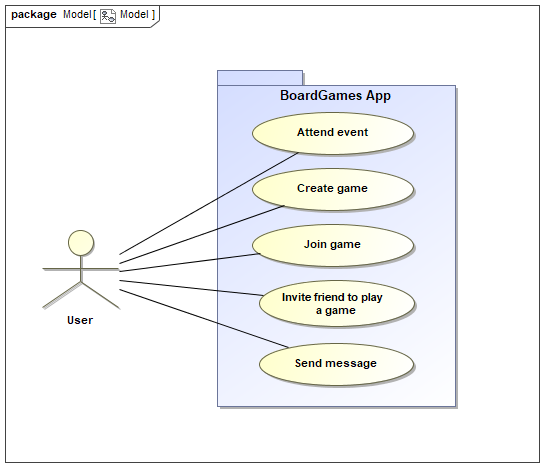
\includegraphics[scale=0.5]{img/UserUseCase}
				\caption{Vartotojo sistemos naudojimo scenarijus}
				\label{img:UserUseCase}
			\end{figure}
			
			\begin{enumerate}
			\item Prisijungti prie žaidimo - vartotojas gali prisijungti prie 
				jau egzistuojančio žaidimo, kuriam įvykti trūksta kelių žaidėjų. (žr. 2 pav.)
				\begin{figure}[H]
					\centering
					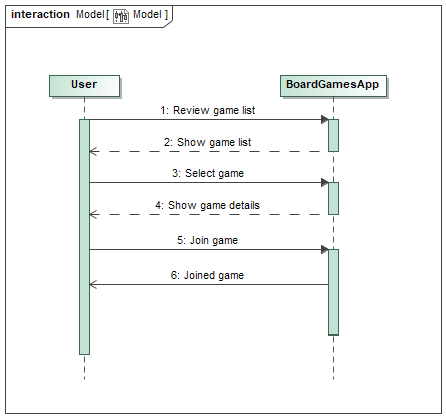
\includegraphics[scale=0.5]{img/JoinGameSequence}
					\caption{Vartotojo prisijungimo prie žaidimo sekų diagrama}
					\label{img:JoinGameSequence}
				\end{figure}
				\textbf{Aprašas:}\\
					Prisijungęs vartotojas gali peržiūrėti jam siūlomus žaidimus, 
					kuriuos yra sukūrę kiti vartotojai. Išsirinkęs žaidimą pagal 
					informaciją, pateiktą su kiekvienu pasiūlymu (žaidimo pavadinimas, 
					vartotojo, sukūrusio žaidimą, vardas ir t.t.), vartotojas jį 
					paspaudžia ir jam parodoma išsamesnė informacija apie žaidimą 
					(jo laikas, vieta, žaidėjų kiekis, aprašymas). Jei visa informacija 
					vartotoją tenkina, jis gali spausti prisijungimo mygtuką. Sistema 
					praneša, apie sėkmingą prisijungimą.
				
			\item Sukurti žaidimą - vartotojas gali inicijuoti privatų arba viešą 
			žaidimą, pasirinkti žaidėjų skaičių, žaidimo vietą, laiką (žr. 3 pav.).
				\begin{figure}[H]
					\centering
					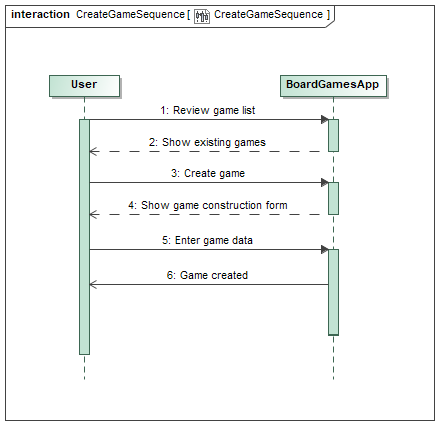
\includegraphics[scale=0.5]{img/CreateGameSequence}
					\caption{Žaidimo kūrimo sekų diagrama}
					\label{img:CreateGameSequence}
				\end{figure}
				\textbf{Aprašas:}\\
					Norėdamas sukurti žaidimą, prisijungęs vartotojas žaidimų sąrašo 
					lange gali pasirinkti kurti žaidimą. Tokiu atveju, jam parodoma 
					žaidimo kūrimo forma, kurioje įrašęs pageidaujamus duomenis 
					(žaidimas, vieta, laikas, žaidėjų skaičius ir t.t), vartotojas ją 
					pateikia. Vartotojas yra informuojamas apie sėkmingą žaidimo sukūrimą.	
					
			\item Pakviesti draugą žaisti - vartotojas gali pakviesti draugą žaisti 
			pasirinktą žaidimą, jei yra pakankamai laisvų vietų (žr. 4 pav.).
				\begin{figure}[H]
					\centering
					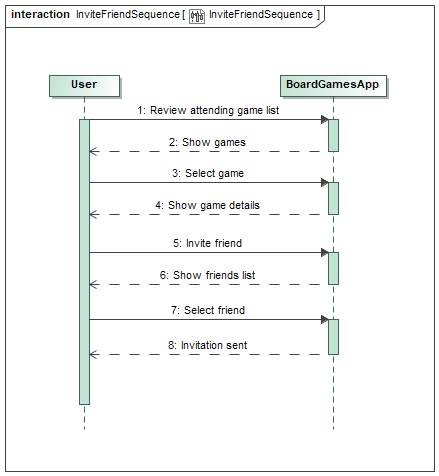
\includegraphics[scale=0.5]{img/InviteFriendSequence}
					\caption{Draugo pakvietimo žaisti sekų diagrama}
					\label{img:InviteFriendSequence}
				\end{figure}
				\textbf{Aprašas:}\\
					Vartotojas, prieš pasirinkdamas prisijungti prie žaidimo, gali 
					pakviesti prie jo prisijungti savo draugą. Vartotojui, 
					pasirinkusiam tam tikrą žaidimą, parodoma platesnė informacija 
					apie jį. Čia vartotojas gali pasirinkti pakviesti draugą - 
					jam parodomas jo draugų sąrašas ir, paspaudus vieną iš draugų, 
					vartotojui pranešama, apie sėkmingą kvietimo išsiuntimą.
				
			\item Parašyti žinutę draugui - vartotojas aplikacijoje gali bendrauti 
			su draugais žinutėmis. (žr. 5 pav.).
				\begin{figure}[H]
					\centering
					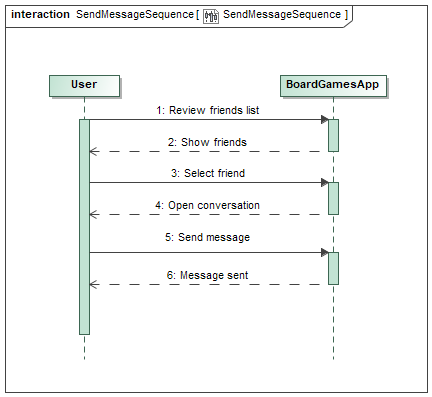
\includegraphics[scale=0.5]{img/SendMessageSequence}
					\caption{Žinutės siuntimo sekų diagrama}
					\label{img:SendMessageSequence}
				\end{figure}
				\textbf{Aprašas:}\\
					Vartotojui suteikiama galimybė peržiūrėti savo draugų sąrašą, 
					pasirinkus vieną ar daugiau draugų, atsidariusiame 
					susirašinėjimų lange, vartotojas gali išsiųsti žinutę.
					
			\item Dalyvauti renginyje - vartotojas gali dalyvauti žaidimų kūrėjų 
			inicijuotame renginyje ar varžybose. (žr. 6 pav.).
				\begin{figure}[H]
					\centering
					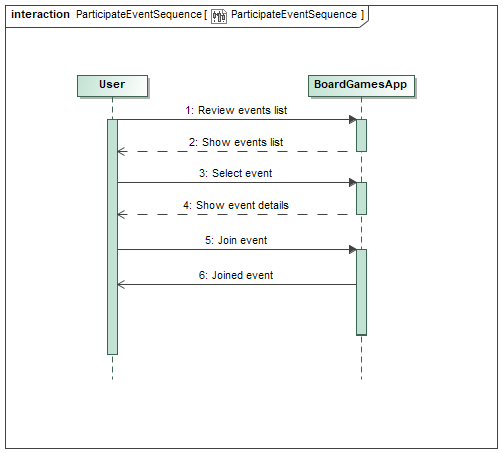
\includegraphics[scale=0.5]{img/ParticipateEventSequence}
					\caption{Vartotojo prisijungimo prie renginio sekų diagrama}
					\label{img:ParticipateEventSequence}
				\end{figure}
				\textbf{Aprašas:}\\
					Vartotojui suteikiama galimybė peržiūrėti savo draugų sąrašą, 
					pasirinkus vieną ar daugiau draugų, atsidariusiame 
					susirašinėjimų lange, vartotojas gali išsiųsti žinutę					
			\end{enumerate}	

		\subsubsubsection {Žaidimų kūrėjo perspektyva}
			\begin{figure}[H]
				\centering
				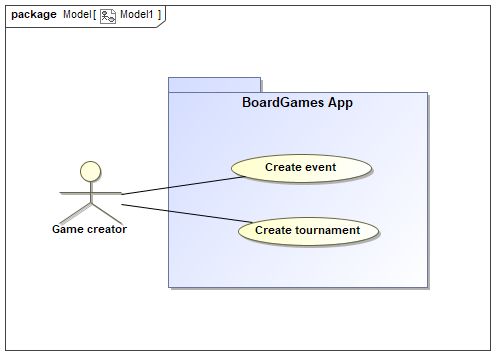
\includegraphics[scale=0.5]{img/CreatorUseCase}
				\caption{Žaidimų kūrėjo scenarijaus sekų diagrama}
				\label{img:CreatorUseCase}
			\end{figure}
			
			\begin{enumerate}
			\item Prisijungti prie žaidimo - vartotojas gali prisijungti prie 
				jau egzistuojančio žaidimo, kuriam įvykti trūksta kelių žaidėjų. (žr. 8 pav.)			
			\item Sukurti žaidimą - vartotojas gali inicijuoti privatų arba viešą 
			žaidimą, pasirinkti žaidėjų skaičių, žaidimo vietą, laiką (žr. 8 pav.).
				\begin{figure}[H]
					\centering
					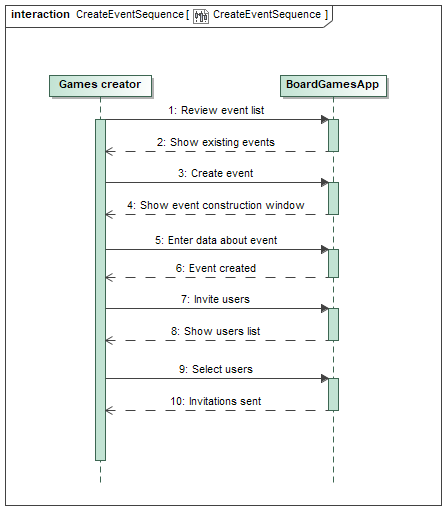
\includegraphics[scale=0.5]{img/CreateEventSequence}
					\caption{Renginio kūrimo sekų diagrama}
					\label{img:CreateEventSequence}
				\end{figure}
				\textbf{Aprašas:}\\
					Žaidimų kūrėjai gali prisijungti prie atskiros paskyros, čia 
					peržiūrėti jau sukurtų žaidimų sąrašą ir pridėti naują renginį. 
					Atsivėrusioje renginio kūrimo formoje kūrėjas turi įvesti 
					pageidaujamus duomenis (renginio vietą, laiką, pobūdį, aprašymą 
					ir t.t.), juos  patvirtinti. Pranešama apie sėkmingą renginio 
					sukūrimą, tada į šį renginį kūrėjas gali kviesti norimus 
					žaidėjus. Jam parodomi jį sekantys žaidėjai, kūrėjas gali 
					pasirinkti kelis ar visus žaidėjus iš sąrašo. Pranešama apie 
					sėkmingai išsiųstus kvietimus.											
			\end{enumerate}		
			
		\subsubsubsection {Administratoriaus}
			\begin{figure}[H]
				\centering
				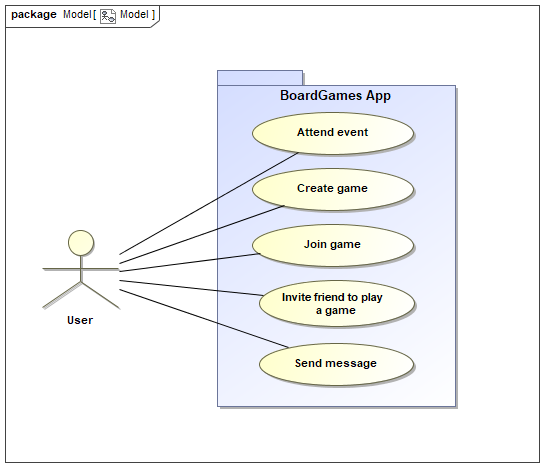
\includegraphics[scale=0.5]{img/UserUseCase}
				\caption{Administratoriaus sistemos naudojimo scenarijus}
				\label{img:UserUseCase}
			\end{figure}
			
			\begin{enumerate}
				\item Trinti žaidimą - administratorius pasilieka teisę trinti 
				taisyklių neatitinkančius žaidimus.
				\item Blokuoti vartotoją - administratorius pasilieka teisę blokuoti 
				taisyklių nesilaikantį vartotoją.
				\item Nutraukti bendradarbiavimą su žaidimų kūrėju - administratorius 
				turi teisę nutraukti kontraktą su žaidimų kūrėju dėl pažeistų platformos taisyklių.			
			\end{enumerate}	
			
	\subsubsection {Sistemos teikiama nauda}
	BoardGames platforma sujungia stalo žaidimų entuziastus, kurie nori žaisti 
	stalo žaidimus neturinčius draugų, žaisiančių konkretų žaidimą, su tais, 
	kuriems trūksta kelių žaidėjų iki pilnos žaidėjų komplektacijos. Taip pat 
	platforma leidžia žaidimų kūrėjų bendrovėms reklamuoti kuriamus žaidimus, 
	rengiant specialius renginius, susitikimus, varžybas, konferencijas. Sistema 
	neabejotinai teikia komercinę naudą žaidimų kūrėjams, jie nesunkiai gali 
	pasiekti tikslinę auditoriją klientams patraukliomis priemonėmis. Kita vertus, 
	sistema padeda žmonėms plėsti savo socialinį akiratį, susirasti bendraminčių 
	ar net draugų. Taip pat sistema supaprastina stalo žaidimų organizavimą vos iki 
	kelių ekrano paspaudimų, todėl tai galima padaryti kaip niekad greitai.	
	
	\subsubsection {Esama būklė}
	Šiuo metu BoardGames komanda turi:
	\renewcommand{\labelitemi}{$\bullet$}
		\begin{itemize}
			\item 5 kompiuterius.
			\item 5 Visual Studio Community programavimo aplinkas.
			\item Telefoną su Android operacine sistema.
			\item Telefoną su IOS.
			\item 3G/4G ryšį mobiliuose įrenginiuose.
			\item Windows forms aplikaciją kūrimo stadijoje.
			\item GitHub repozitoriją.
		\end{itemize}	

	\subsubsection {Priemonės scenarijui įgyvendinti}
	Priemonės, kurių BoardGames komandai trūksta tikslingam programos įgyvendinimui:
	\renewcommand{\labelitemi}{$\bullet$}
		\begin{itemize}
			\item Privati Git repozitorija.
			\item Duomenų bazė.
			\item Serveris aplikacijos api talpinti.
			\item Patyrę programuotojai aplikacijai sukurti.
			\item Rinkodaros strategija.
			\item Numatytos lėšos aplikacijos talpinimui skirtingų platformų aplikacijų parduotuvėse.
		\end{itemize}	
\subsection {Įgyvendinamumo ir naudos analizė}		
	\subsubsection{Operacinis įgyvendinamumas}
		\noindent \textbf{Problema} Klientai gali nesinaudoti programėle, nes gali manyti, kad esančios alternatyvos (socialiniai tinklai (pvz. “Facebook”) yra patogesni.\\
		\noindent \textbf{Problemos sprendimas} Akcentuoti programėlės patogumą ir paprastumą. \\

		\noindent \textbf{Problema} Klientai gali nesinaudoti programėle, nes gali manyti, kad neverta jos siųstis, jei ja planuoja naudotis tik kelis kartus. \\
		\noindent \textbf{Problemos sprendimas} Stengtis pernelyg daug neišplėsti programėlės funkcionalumo, padaryti programėlę paprastą, kad ji užimtų ne daug vietos telefone. Be to, būtų numatytas ir alternatyvios web aplikacijos sukūrimas, kuri naudotų tą patį serverio API, todėl susirasti ar sukurti žaidimą būtų galima tiesiog naudojant naršyklę.\\
		
		\noindent \textbf{Problema} Nors vienas sėkmingo programėlės naudotojo apgavimo atvejis, paskelbtas viešai, galėtų tapti programėlės gyvavimo ir pačio projekto pabaiga dėl teisinių institucijų reikalavimo uždaryti/riboti veiklą.\\
		\noindent \textbf{Problemos sprendimas} Būtina įvesti tam tikro lygio vartotojų identifikaciją siekiant užtikrinti, jog tiek kuriantys, tiek ir prisijungiantys žmonės žinotų, su kuo turi reikalų. Taip pat galima įvesti reitingavimo, atsiliepimų sistemas, kurios leistų lengvai nustatyti įtartinos reputacijos naudotojus, kuriančius (hosting) žaidimo sesijas ar prie jų norinčius prisijungti. Įvykdžius pastaruosius reikalavimus programėlė pasižymėtų socialiniu saugumu, o tai reklamuojant galima išgauti strateginį pranašumą prieš galimus konkurentus.\\
		
		\noindent \textbf{Problema} Mobilioji programėlė taikoma į labai ribotą ir tikslinę auditoriją – tai žmonės, kurie itin mėgsta stalo žaidimus. Ši pastaba leidžia daryti prielaidą, jog didžioji dalis potencialių vartotojų būtų jaunesnio amžiaus ir/arba vyresni žmonės, kurie labiau mėgsta anime kultūrą, loginį mąstymą.\\
		\noindent \textbf{Problemos sprendimas} Itin tikslinga ir siaura auditorija yra labai paranki, nes leidžia labiau numatyti potencialių vartotojų elgseną, pomėgius, todėl vykdant reklamines kampanijas galima lengviau pasiekti naują vartotoją. Taip pat galimybė tartis su įvairių stalo žaidimų kūrėjais dėl partnerystės galimybių. Pvz. programėlės naudotojas per ją tiesiogiai sužino apie naują stalo žaidimą, užsinori jį įsigyti, tai gali padaryti programėlės pagalba, su kuria pvz. jis gautų tam tikrą nuolaidą, o mes – programėlės kūrėjai – galime susitarti dėl papildomo finansavimo ar komisinių galimybės iš stalo žaidimų kūrėjų. Dėl tikslingos auditorijos žaidimų įsigyjimo konversijos rodiklis būtų aukštas.\\
		
		\noindent \textbf{Problema} Tam tikrais laiko tarpais bei aplikacijos išleidimo pradžioje gali trūkti vartotojų, todėl programėlės užimtumas bus labai mažas ir ilgai truks pradėti naujus žaidimus.\\
		\noindent \textbf{Problemos sprendimas} Leisti vartotojams prisijungti naudojantis dabartiniais socialiniais tinklais ir pakviesti juose esančius draugus parsisiųsti programėlę. Vartotojai, sudalyvavę žaidime pirmomis išleidimo savaitėmis, galėtų gauti prizų. \\
		
		\noindent \textbf{Problema} Labai maža klientų dalis gali pirkti paslaugą, skirtą iškelti kuriamą žaidimą bendrame žaidimų sąraše.\\
		\noindent \textbf{Problemos sprendimas} Samdyti marketingo specialistą, kuris padėtų programėlės vartotojus įtikinti mokamos paslaugos svarba. \\
		
		\noindent \textbf{Problema} Vartotojai gali neapsilankyti programėlėje ilgą laiko tarpą.\\
		\noindent \textbf{Problemos sprendimas} Įgyvendinti funkcionalumą, kuris vartotojui skirtų prizą įsijungus aplikaciją bent kartą kiekvieną dieną. Epizodiškai siųsti vartotojui pranešimus apie netoli jo įvyksiantį žaidimą, kurį vartotojas yra įtraukęs į savo mėgstamų žaidimų sąrašą arba žaidimą, kuriame dalyvauja vartotojo draugai, su kvietimu prisijungti prie jo. Reklamuojant programėlę, bandyti įtikinti vartotojus, kad jie pakviestų savo draugus įsitraukti į programėlės veiklą ir taip sukurti naudotojų mėgstamą laisvalaikio praleidimo formą, kurią jie naudotų reguliariai.\\
		
		\noindent \textbf{Problema} Vartotojo operacinė sistema gali būti atgyvenusi.\\
		\noindent \textbf{Problemos sprendimas} Suprogramuoti aplikaciją taip, kad ji būtų prieinama kuo didesniam operacinių sistemos versijų diapazonui.\\
		
		\noindent \textbf{Problema} Sistemos sukūrimas. Pasamdyti darbuotojai gali neišpildyti visų norimų reikalavimų.\\
		\noindent \textbf{Problemos sprendimas} Tam, kad sistema būtų sukurta tiksliai tokia, kokios reikalaujame, darbuotojams bus iškelti aiškūs nurodymai, sudaryti pagal reikalavimų dokumentą. \\
		
		\noindent \textbf{Problema} Sklandaus sistemos veikimo užtikrinimas. Tiek dėl pačios sistemos, tiek dėl vartotojų klaidų sistema gali pateikti netikslią informaciją. \\
		\noindent \textbf{Problemos sprendimas} Tam, kad būtų sumažinti sistemos netikslumai, bus samdomi darbuotojai, kurie nuolat testuos ir sieks kuo patogesnio bei tikslesnio veikimo.\\
		
		\noindent \textbf{Problema} Sistemoje gali likti senų, nereikalingų duomenų, galinčių sudaryti sunkumų naudotojams, siekiantiems prisijungti prie žaidimo. \\
		\noindent \textbf{Problemos sprendimas} Sistemoje bus įdiegta programa, kuri automatiškai po tam tikro laiko panaikins galimybę prisijungti prie jau pasibaigusio žaidimo ir kitus nebereikalingus duomenis. \\
		
		\noindent \textbf{Problema}  Į silpną sistemą gali įsilaužti nepageidaujami asmenys.\\
		\noindent \textbf{Problemos sprendimas} Tam, kad į sistemą nebūtų įsilaužta ir ji nebūtų pažeista, bus samdomi darbuotojai, užtikrinantys sistemos saugumą.  \\
		
	\subsubsection{Techninis įgyvendinamumas}
		\noindent \textbf{Problema} Sistemos veikimas bus paremtas integruoto GPS įrenginio naudojimu bei interneto ryšiu. Dauguma išmaniųjų įrenginių turi GPS paruoštą naudojimui, todėl ši sistema techniškai įgyvendinama. Kadangi žaidimas vyks miesto ribose, dėl interneto problemų kilti neturėtų. \\
		\noindent \textbf{Problemos sprendimas} Sklandžiam veikimui užtikrinti galima duomenis kešuoti, tada sistema bus mažiau pririšta prie interneto.\\
		
		\noindent \textbf{Problema} Esamam personalui trūksta serverių priežiūros, duomenų bazių valdymo, internetinių svetainių bei mobiliųjų aplikacijų kūrimo ir panašių įgūdžių.\\
		\noindent \textbf{Problemos sprendimas} Personalo apmokymas, internetinių video pamokų portalų paslaugų prenumeratų įsigijimas, individualus darbuotojų mokymasis, ekspertų pagalba. \\	
		
		\noindent \textbf{Problema} Serveriui, internetinei svetainei ir mobiliajai aplikacijai reikia nuolatinės priežiūros, kad duomenys visada būtų validūs, o serveris veiktų efektyviai ir vartotojui būtų malonus naudoti.\\
		\noindent \textbf{Problemos sprendimas} Specialistų samdymas serverių techninei priežiūrai, gera backend sistema lengvai programėlės internetinės svetainės bei programėlės priežiūrai ir duomenų įvedimui, išėmimui bei keitimui. \\
		
		\noindent \textbf{Problema} Programėlės naudotojai, norintys teikti žaidimų pasiūlymus, turi užsiregistruoti programėlėje ir pasirinktinai pateikti savo asmeninius duomenis. Jei nebus užtikrintas sistemos saugumas, privatūs duomenys gali būti nutekinti.\\
		\noindent \textbf{Problemos sprendimas} Samdyti duomenų saugumo specialistus, apmokyti darbuotojus, kad būtų laikomasi gerų programavimo praktikų, užtikrinančių duomenų saugumą kuriamoje sistemoje. \\
		
		\noindent \textbf{Problema} Užsisakant žaidimo iškėlimą sistemoje piniginės transakcijos gali būti perimtos trečių šalių asmenų ir vartotojo pinigai gali būti nesaugiai perduodami organizacijai.\\
		\noindent \textbf{Problemos sprendimas} Bendradarbiavimas su bankais, piniginių transakcijų vykdymas per jų sistemas, taip užtikrinant vartotojų pinigų saugumą. \\
		
		\noindent \textbf{Problema} Laikui bėgant serveriuose neišvengiamai kaupsis vis daugiau informacijos: vartotojų duomenų, žaidimų įrašų ir pan. Paprastas komunikavimas su serveriu taps nepakankamai efektyvus ir užtruks per daug laiko.\\
		\noindent \textbf{Problemos sprendimas} Pasirūpinti efektyvių algoritmų analize ir įgyvendinimu, kad sistema galėtų efektyviai dirbti su milžinišku kiekiu duomenų ir vartotojas nepajustų jokių šalutinių efektų. \\
		
	\subsubsection{Ekonominis įgyvendinamumas}	
		Programėlės išleidimas skaičiuojamas taip: 21,12 € (išleidimo į Google 
		Play Store kaina) + 83.63 € / m. (išleidimo į Apple Store kaina)  + 10,13 
		€ / m. (išleidimo į Microsoft Store kaina).
		
		Mobiliosios aplikacijos sukūrimo kainos formulė: 5 dirbantys žmonės * 20 
		darbo dienų (mėnuo) * 4 valandos * 15 € (valandinis užmokestis 
		programuotojui).

		Aplikacijos palaikymas skaičiuojamas taip: 1 dirbantis žmogus * 8 valandos * 4 
		savaitės * 5,13 € (vidutinis valandinis užmokestis Lietuvoje).

		Marketingo specialisto samdymo kaina skaičuojama taip: 1 dirbantis žmogus * 
		10 valandų * 4 savaitės * 5,13 € (vidutinis valandinis užmokestis Lietuvoje).

		Taip pat turime įtraukti ir lėšas, kurios bus skiriamos apmokėti SEO 
		agentūros darbą siekiant iškelti svetainę paieškos sistemos rezultatų 
		puslapiuose. Kadangi potencialus srautas 1 mln. Paieškų per mėnesį visame 
		pasaulyje, todėl reikės didelės agentūros nuolatinio darbo, kaštai - 
		500/mėn. * 12 (tikime, jog SEO agentūra rezultatą pasieks per metus) = 
		6000€ (per dvejus metus)

		Techninės įrangos kaina skaičiuota taip: Kompiuterių kaina (2 * 2 000 = 
		4 000 €) + Telefonų kaina (3 * 400 = 1 200 €).
		
		\begin{longtable}{ | m{8cm} | m{8cm} | }
		\caption{Išlaidos}
		\label{variability_impl_mech}
		%\endfirsthead
		\endhead
		 \hline			

		\textbf{Dalykas} & \textbf{Kaina} \tabularnewline \hline
		Programėlės išleidimas. & 21,12 € + 93,76 € / met. \tabularnewline \hline
		Mobiliosios aplikacijos sukūrimo kaina. & 6000 € \tabularnewline \hline
		Aplikacijos palaikymas. & 164,16 € / mėn. \tabularnewline \hline
		Serverių nuoma & 80 € / mėn. \tabularnewline \hline
		Marketingas. & 505,2 € / mėn. \tabularnewline \hline
		Techninė įranga. & 5200 €  \tabularnewline \hline
		Domeno išpirka. & 10 € / met. \tabularnewline \hline
		\end{longtable}
		
		Bendros išlaidos per 2 metus skaičiuojamos taip (mėnesinės išlaidos 
		dauginamos iš 20 mėnesių, nes 4 mėnesius bus kuriama aplikacija) : 
		techninė įranga (5200 €) + aplikacijos sukūrimo kaina (6000 €) +  
		programėlės išleidimo kaina (21,12 € + 93,76 € * 2 metai = 208,64 €) + 
		aplikacijos palaikymo kaina (164,16 € * 20 mėn. = 3283,2 €) +  serverių 
		nuomos kaina (80 € * 20 mėn. = 1600 €) + marketingo kaina (505,2 € * 20 
		mėn. = 10104 €) + domeno išpirkos kaina (2 * 10 €). Iš čia gauname, kad 
		bendros išlaidos iš viso kainuos 26415,84 €.
		
		\begin{figure}[H]
			\centering
			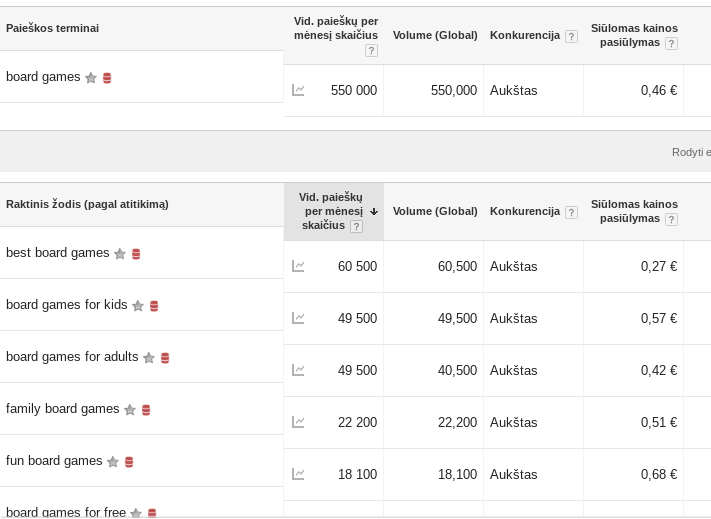
\includegraphics[scale=0.5]{img/economics}
			\caption{Renginio kūrimo sekų diagrama}
			\label{img:economics}
		\end{figure}
		
		Maksimali galima globali auditorija paieškos tinkluose: 1 mln. Paieškų per 
		mėnesį (atsižvelgiame tik į Google sistemą, nes ji užima didžiąją rinkos 
		dalį). Pasitelkus SEO (Search Engine Optimisation) specialistus, marketingo 
		ir turinio rašymo ekspertus, galima tikėtis pasiekti \#7 - \#10 pozicijas 
		pirmame paieškos rezultatų puslapyje. Esant tokioms pozicijoms, yra 
		nustatyta, jog svetainė generuoja 1,5 - 3,5% paspaudimų nuo visų paieškų 
		skaičiaus per mėnesį (vidurkis: 2,5%). Taigi, po 2 metų galime tikėtis, 
		jog per vieną mėnesį iš natūralaus paieškos srauto mūsų web aplikaciją 
		aplankytų 25000 unikalių vartotojų visame pasaulyje. Konversijos tipas 
		svetainėje - mobiliosios programėlės atsisiuntimas. Kadangi šie lankytojai 
		- gana tikslinė auditorija, todėl nustatėme, jog realus konversijos 
		procentas: 5%. Taigi, vien iš paieškos srauto, būtų galima pritraukti apie 
		1250 naujų programėlės parsisiuntimų per mėnesį.

		Svetainėje galima įdiegti Google Adwords reklamos banerinius laukus, 
		kurių vidutinis konversijos rodiklis: 4% nuo unikalių lankytojų, o 
		vidutinis užmokestis už paspaudimą - 0,02€
		Todėl vien svetainė per po 2 metų galėtų generuoti 25000 * 0,04 * 
		0,02 = 20€ per mėnesį.

		Manome, kad mobiliąją aplikaciją per mėnesį atsisiųs apie 500 (paieškos 
		Google Play Store, App Store, Microsoft Store) + 1250 (paieškos tinklai) 
		+ 200 (socialiniai tinklai) = 1950 žmonių. Tikėtina, kad apie 5% žmonių 
		paspaus ant reklamos nuorodos naudojantis programėle. Taip pat tikėtina, 
		kad vartotojai dėl dienos prizų aplikacijoje apsilankys apie 15 kartų per 
		mėnesį. Taigi, pirmą mėnesį iš reklamų bus galima užsidirbti 1950 * 15 * 
		0.05 * 0.02 € = 29,25€. Pagal aritmetinę progresiją po 2 metų (20 mėnesių, 
		kai bus išleista aplikaciją), iš reklamų bus galima uždirbti: (20 * ( 49,25 
		+ 49,25 * 20)) / 2 = 10342,5 €.

		Programėlė pinigus galės uždirbti ne tik iš paprastų reklamų, bet ir 
		iš rėmėjų, kurie užsiima stalo žaidimų prekyba. Tikėtina, kad programėlė 
		nuolat turės apie 3 rėmėjus, iš kurių bus galima gauti apie 1500 € lėšų 
		per metus. Taigi, per 2 metus programėlė iš rėmėjų turėtų gauti 3 * 2 * 
		1500 € = 9000 €.

		Taip pat manome, kad aplikacijoje apie 5% aktyvių vartotojų naudosis 
		žaidimo iškėlimo paslauga ir pirks ją bent kartą į mėnesį. Tikėtina, kad 
		aplikacija turės apie 2000 aktyvių vartotojų. Taigi, per 2 metus būtų 
		galima surinkti: 20 * 2000 * 0,05 * 1.49 = 2980 €.

		Žaidimo iškėlimo paslauga: tai galimybė 3 kartus iškelti žaidimą bendrame
		žaidimų sąraše, padėsianti daug greičiau surinkti visus žaidimui prasidėti 
		trūkstamus žaidėjus. Žaidėjas, nusipirkęs tokią paslaugą, gali pasinaudoti 
		ja bet kuriam jo sukurtam žaidimui. Jos kaina - 1.49 € arba 500 žaidimo 
		monetų.

		\begin{longtable}{ | m{10cm} | m{6cm} | }
		\caption{Pajamos}
		\label{variability_impl_mech}
		%\endfirsthead
		\endhead
		 \hline			

		\textbf{Pajamų šaltinis} & \textbf{Numatoma suma per 2 metus} \tabularnewline \hline
		Rėmėjų skiriamos lėšos mainais už teikiamą reklamą. & 9000 € \tabularnewline \hline
		Vartotojų išpirkta paslauga skirta iškelti žaidimą aukščiau bendrame sąraše. & 2980  € \tabularnewline \hline
		Reklamos mobiliojoje aplikacijoje ir svetainėje. & 10342,5 €\tabularnewline \hline
		\end{longtable}
		
		Iš viso aplikacija per 2 metus turėtų užsidirbti 9000 € + 2980 € + 10342,5 €
		= 22322 €.

		Gauname, kad projektas per 2 metus neatsipirks: 22322 € - 26415,84 € = 
		-4093,84 €. Vis dėlto, programėlė jau sukurta, o įranga nupirkta, todėl 
		už tai papildomų išlaidų mokėti nebereiks ir programėlė, praėjus kiek 
		daugiau laiko, pradės atsipirkti (trečiaisiais metais bus veikla jau bus 
		pelninga).
		
	\subsubsection{Juridinis įgyvendinamumas}
		Programėlės kūrėjai užtikrina vartotojų asmeninių duomenų saugumą. 
		Veiklos vystymas turės būti įformintas viena iš galimų verslo formų, 
		pvz.: UAB, MB ar kt., todėl būtinas įsiregistravimas į Valstybinę 
		duomenų apsaugos inspekciją, kuri patikros būdu užtikrins, jog 
		programėlės veikla atitinka vartotojų duomenų apsaugos reglamentus, 
		t.y. Duomenys kaupiami ir apdorojami tvarkingai, yra patikimai saugomi, 
		nėra grėsmės juos atskleisti nepageidaujamiems tretiems asmenims.
		
\subsection{Išvada}
	Dalykinės srities verslo proceso analizė yra vieną svarbiausių viso projekto 
	sudedamųjų dalių. Išsamus ir tikslus šios dalies aprašas leidžia tinkamai 
	įvertinti planuojamos kurti sistemos finansinį, teisinį, technologinį 
	pagrįstumą ir priimti lemiamą išvadą - vystyti projektą ar atsisakyti 
	numatomo sistemos plano. Teisingas sprendimas šioje stadijoje leidžia 
	išgauti ilgalaikę finansinę naudą arba betikslių išlaidų prevenciją, o 
	klaidingas - nulemia tolimesnius, automatiškai destruktyvius sprendimus, 
	lemsinčius projekto žūtį. Net ir menki netikslumai šioje projekto eigoje 
	gali lemti iškraipytą bendrą sistemos verslo vaizdą. Atlikus šį tyrimą ir 
	nusprendus, jog sistema pagrįsta visais anksčiau nurodytais aspektais, galima 
	pradėti formuoti jos pagrindus, t.y. Apibrėžti formalius reikalavimus.

\section{Reikalavimų specifikacija}

\subsection{Įvadas}

Programėlės vartotojai: 
\begin{itemize}
	\item Stalo žaidimų mėgėjai
	\item Stalo žaidimų kūrimo kompanijos
\end{itemize}

Stalo žaidimų mobilioji programėlė yra projektas, skirtas išaudoti dar neužpildytą nišą mobiliųjų programėlių versle, sukuriant nemokamą, reklama pagrįstą programėlę, skirtą stalo žaidimų mėgėjams. 
Šio antrojo laboratorinio darbo paskirtis yra susipažinti su kuriamos sistemos achitektūros reikalavimų (funkcinių, nefunkcinių, vartotojo sąsajos) sudarymo eiga ir detalėmis.

\subsection{Funkciniai reikalavimai asmeninio vartotojo perspektyva}
Šiame skyriuje pateikiami sistemos funkciniai reikalavimai, t.y. pagrindinės sistemos atliekamos funkcijos, konkretūs jų aprašymai.

\newcounter{frcount}
\newcommand\rownumberfr{\stepcounter{frcount}\arabic{frcount}}

\subsubsection{Aplikacijos langai}
\begin{longtable}{ | >{\centering}m{2cm} | m{10cm} | >{\centering}m{2.5cm} | } \caption{Aplikacijos langai.} \endhead \hline
\multicolumn{3}{ |l| }{\textbf{Aplikacijos langai:}} \tabularnewline \hline
\textbf{Numeris} & \centering{\textbf{Reikalavimas}} & \textbf{Svarba} \tabularnewline \hline
FR\rownumberfr & Registracija - šiame lange vartotojas gali prisiregistruoti prie programėlės. & Būtina\tabularnewline \hline
FR\rownumberfr & Prisijungimas - šiame lange vartotojas gali prisijungti prie programėlės. & Būtina\tabularnewline \hline
FR\rownumberfr & Pagrindinis langas - iš šio lango vartotojas gali pasirinkti, kokias veiklas nori veikti programėlėje. & Būtina\tabularnewline \hline
FR\rownumberfr & Žaidimų pasirinkimo langas - šiame lange vartotojas gali matyti galimus žaidimus ir prie jų prisijungti. & Būtina\tabularnewline \hline
FR\rownumberfr & Žaidimo kūrimo langas - šiame lange vartotojas gali sukurti žaidimą ir pateikti informaciją apie jį. & Būtina\tabularnewline \hline
FR\rownumberfr & Žaidimų išėlimo langas - šiame lange vartotojas gali nustatyti, kiek ilgai nori, kad jo žaidimas būtų išeltas žaidimų sąrašo viršuje. & Būtina\tabularnewline \hline
FR\rownumberfr & Draugų sąrašas - šiame lange vartotojas gali matyti savo draugų sąrašą, taip pat prisijungusius draugus. & Būtina\tabularnewline \hline
FR\rownumberfr & Žaidimo langas - šis langas rodomas vartotojui prisijungus prie žaidimo. Jame galima pasiekti pilną informaciją apie žaidimą ir susirašinėti su komandos nariais. & Būtina\tabularnewline \hline
FR\rownumberfr & Vartotojo profilio langas - šiame lange rodomi vartotojo profilio duomenys, juos galima redaguoti. & Būtina\tabularnewline \hline
FR\rownumberfr & Mano žaidimų langas - šiame lange bus rodomi visi žaidimai, kuriuos vartotojas yra sukūręs ir žaidimai, prie kurių jis yra prisijungęs. & Būtina\tabularnewline \hline
\end{longtable}

\subsubsection{Registracija}
\begin{longtable}{ | >{\centering}m{2cm} | m{10cm} | >{\centering}m{2.5cm} | } \caption{Funkciniai registracijos reikalavimai asmeninio vartotojo perspektyva.} \endhead \hline
\multicolumn{3}{ |l| }{\textbf{Registracija:}} \tabularnewline \hline
\textbf{Numeris} & \centering{\textbf{Reikalavimas}} & \textbf{Svarba} \tabularnewline \hline
FR\rownumberfr & Pradiniame lange, paspaudus mygtuką “Registracija asmeniui”, atsiveria registracijos anketa. & Būtina\tabularnewline \hline
FR\rownumberfr & Suteikiama galimybė registruotis per Facebook, Google paskyras arba elektroniniu paštu. & Būtina\tabularnewline \hline
FR\rownumberfr & Registruojantis vartotojas privalo nurodyti prisijungimo vardą, slaptažodį gimimo metus, elektroninį paštą ir gali pateikti nuotrauką. & Būtina\tabularnewline \hline
FR\rownumberfr & Jei norimas vartotojo vardas jau egzistuoja, vartotojui reikia įvesti naują vartotojo vardą. & Būtina\tabularnewline \hline
FR\rownumberfr & Tikrinama, ar elektroninis paštas yra validus (baigiasi simboliu ‘@’ ir domenu) ir ar jis egzistuoja. Jei elektroninis paštas netinkamas, vartotojui turi būti apie tai pranešama ir paprašoma duomenis įvesti iš naujo. & Būtina\tabularnewline \hline
FR\rownumberfr & Registruojantis vartotojas yra prašomas pakartoti slaptažodį du kartus. & Būtina\tabularnewline \hline
FR\rownumberfr & Vartotojas registracijos metu turi sutikti su aplikacijos naudojimosi sąlygomis prieš tai jas peržiūrėjęs. & Būtina\tabularnewline \hline
FR\rownumberfr & Jei visi duomenys įvesti teisingai, jie turi būti išsaugomi duomenų bazėje, vartotojui turi būti praneša apie sėkmingą registraciją. & Būtina\tabularnewline \hline
FR\rownumberfr & Vartotojui sėkmingai užsiregistravus (el. pašto būdu) išsiunčiamas patvirtinimo laiškas nurodytu elektroninio pašto adresu. Vartotojas turi paspausti patvirtinimo nuorodą, jog registracija būtų užbaigta. & Būtina\tabularnewline \hline
\end{longtable}

\subsubsection{Prisijungimas}
\begin{longtable}{ | >{\centering}m{2cm} | m{10cm} | >{\centering}m{2.5cm} | } \caption{Funkciniai prisijungimo reikalavimai asmeninio vartotojo perspektyva.} \endhead \hline
\multicolumn{3}{ |l| }{\textbf{Prisijungimas:}} \tabularnewline \hline
\textbf{Numeris} & \centering{\textbf{Reikalavimas}} & \textbf{Svarba} \tabularnewline \hline
FR\rownumberfr & Vartotojas gali prisijungti per Facebook, Google paskyras arba lokaliai. & Būtina\tabularnewline \hline
FR\rownumberfr & Prisijungimo lokaliai metu vartotojas gali pasirinkti, ar įvesti vartotojo vardą, ar elektroninio pašto adresą, ir privalo įvesti slaptažodį. & Būtina\tabularnewline \hline
FR\rownumberfr & Programėlė tikrina, ar vartotojo vardas ir slaptažodis įvesti teisingai, jei ne, tai turi būti praneša vartotojui ir paprašoma iš naujo įvesti duomenis. & Būtina\tabularnewline \hline
FR\rownumberfr & Jei vartotojas buvo prisijungęs prie žaidimo ir neatsijungė, kitus kartus jis prijungiamas paleidus programėlę be duomenų įvedimo. & Būtina\tabularnewline \hline
FR\rownumberfr & Prisijungęs vartotojas gali  atsijungti ir suteikiama galimybė prisijungti kitam vartotojui. & Būtina\tabularnewline \hline
FR\rownumberfr & Vartotojui pamiršus slaptažodį, jis gali būti pakeičiamas naudojantis elektroniniu paštu. Vartotojas gali pateikti prašymą pakeisti slaptažodį, tada į jo paštą bus atsiunčiamas laišas su nauju slaptažodžiu ir nuoroda, patvirtinančia operaciją. & Būtina\tabularnewline \hline
\end{longtable}

\subsubsection{Pagrindinis langas}
\begin{longtable}{ | >{\centering}m{2cm} | m{10cm} | >{\centering}m{2.5cm} | } \caption{Funkciniai pagrindinio lango reikalavimai asmeninio vartotojo perspektyva.} \endhead \hline
\multicolumn{3}{ |l| }{\textbf{Pagrindinio lango reikalavimai:}} \tabularnewline \hline
\textbf{Numeris} & \centering{\textbf{Reikalavimas}} & \textbf{Svarba} \tabularnewline \hline
FR\rownumberfr & Vartotojas gali patekti į egzistuojančių žaidimų sąrašą. & Būtina\tabularnewline \hline
FR\rownumberfr & Vartotojas gali patekti į savo draugų sąrašą. & Būtina\tabularnewline \hline
FR\rownumberfr & Vartotojas gali patekti į žaidimo kūrimo langą. & Būtina\tabularnewline \hline
FR\rownumberfr & Vartotojas gali patekti į paskyros nustatymų langą. & Būtina\tabularnewline \hline
FR\rownumberfr & Vartotojas gali atsijungti. & Būtina\tabularnewline \hline
\end{longtable}

\subsubsection{Žaidimų pasirinkimo langas}
\begin{longtable}{ | >{\centering}m{2cm} | m{10cm} | >{\centering}m{2.5cm} | } \caption{Funkciniai žaidimų pasirinkimo lango reikalavimai asmeninio vartotojo perspektyva.} \endhead \hline
\multicolumn{3}{ |l| }{\textbf{Žaidimų pasirinkimo lango reikalavimai:}} \tabularnewline \hline
\textbf{Numeris} & \centering{\textbf{Reikalavimas}} & \textbf{Svarba} \tabularnewline \hline
FR\rownumberfr & Vartotojas gali filtruoti žaidimus pagal miestą, žaidimą, žaidimo kategoriją, trūkstamų žaidėjų skaičių, žaidimų kūrėjo reitingą, užsiregistravusių žaidėjų reitingų vidurkį ir atstumo spindulį, esantį tarp vartotojo ir vietos, kurioje vyks žaidimas, numatomą žaidimo pradžios laiką. & Būtina\tabularnewline \hline
FR\rownumberfr & Vartotojas gali filtruoti žaidimus pagal kelis raktus. & Būtina\tabularnewline \hline
FR\rownumberfr & Pasirinkęs žaidimą, vartotojas gali peržiūrėti platesnę žaidimo informaciją, pateikti prašymą prisijungti prie siūlomų stalo žaidimų sesijų ar palikti žaidimą, prie kurio jau buvo prisijungęs. & Būtina\tabularnewline \hline
FR\rownumberfr & Jei žaidime nebėra laisvų vietų, žaidimas sąraše nėra rodomas. & Būtina\tabularnewline \hline
FR\rownumberfr & Jei žaidimo numatytas pradžios laikas jau yra praėjęs, tuomet jis žaidimų sąraše nerodomas. & Būtina\tabularnewline \hline
\end{longtable}

\subsubsection{Žaidimo kūrimo langas}
\begin{longtable}{ | >{\centering}m{2cm} | m{10cm} | >{\centering}m{2.5cm} | } \caption{Funkciniai žaidimo kūrimo lango reikalavimai asmeninio vartotojo perspektyva.} \endhead \hline
\multicolumn{3}{ |l| }{\textbf{Žaidimo kūrimo langas:}} \tabularnewline \hline
\textbf{Numeris} & \centering{\textbf{Reikalavimas}} & \textbf{Svarba} \tabularnewline \hline
FR\rownumberfr & Vartotojas gali pats sukurti stalo žaidimo sesiją. & Būtina\tabularnewline \hline
FR\rownumberfr & Kuriant žaidimą, vartotojas privalo nurodyti žaidimo pavadinimą, minimalų ir maksimalų žaidėjų skaičių, žaidimo vietą. & Būtina\tabularnewline \hline
FR\rownumberfr & Kuriant žaidimą, vartotojas gali nurodyti neprivalomus duomenis: tikėtiną žaidimo pradžios laiką, žaidimo aprašymą. & Būtina\tabularnewline \hline
FR\rownumberfr & Vartotojas gali pašalinti žaidimą iš jo jau sukurtų žaidimų sąrašo. & Būtina\tabularnewline \hline
FR\rownumberfr & Vartotojas gali visuomet keisti savo sukurto žaidimo duomenis. & Būtina\tabularnewline \hline
FR\rownumberfr & Jei žaidimo duomenys pakeičiami, prisijungę žaidėjai apie tai įspėjami automatine žinute su informacija apie pakeitimus, kuri pasirodo žaidimo susirašinėjimo gijoje. & Būtina\tabularnewline \hline
FR\rownumberfr & Atsiradus naujam vartotojui, norinčiam prisijungti prie sukurto žaidimo, vartotojas, sukūręs žaidimą, gali priimti arba atmesti šį prašymą. & Būtina\tabularnewline \hline
FR\rownumberfr & Žaidimą sukūręs vartotojas gali pats pasiūlyti kitiems žaidėjams prisijungti prie jo kuriamo žaidimo spausdamas mygtuką “+” ir nurodydamas kitų žaidėjų prisijungimo vardus. & Būtina\tabularnewline \hline
FR\rownumberfr & Jei įvestas žaidėjas neegzistuoja, aplikacija informuoja žaidimą sukūrusį vartotoją, kad toks žaidėjas neegzistuoja. & Būtina\tabularnewline \hline
FR\rownumberfr & Jeigu įvestas žaidėjas žaidimo nurodytu pradžios metu jau yra prisijungęs prie kito žaidimo, aplikacija informuoja žaidimą sukūrusį vartotoją, kad šis žaidėjas šiuo metu negali dalyvauti žaidime. & Būtina\tabularnewline \hline
FR\rownumberfr & Žaidimą sukūręs vartotojas bet kada gali išmesti žaidėją iš savo žaidimo. & Būtina\tabularnewline \hline
FR\rownumberfr & Įvedus visą reikiamą informaciją apie žaidimą spaudžiamas mygtukas “Sukurti”. & Būtina\tabularnewline \hline
FR\rownumberfr & Sukūrus žaidimą, vartotojai, pakviest prisijungti prie žaidimo, turi patvirtinti, kad sutinka prisijungti. & Būtina\tabularnewline \hline
FR\rownumberfr & Kol pakviestas vartotojas nėra patvirtinęs prisijungimo prie žaidimo, šalia vaizduojama būsena “Laukia patvirtinimo”. & Būtina\tabularnewline \hline
FR\rownumberfr & Jei pakviestas vartotojas atmeta pakvietimą, jo vardas dingsta iš žaidėjų sąrašo. & Būtina\tabularnewline \hline
FR\rownumberfr & Šalia žaidimą sukūrusio vartotojo vardo vaizduojama būsena “Šeimininkas”. & Būtina\tabularnewline \hline
FR\rownumberfr & Jeigu norima žaidimą iškelti visų žaidimų sąraše į viršų, galima už papildomą mokestį įsigyti tokią paslaugą. Vartotojas, suinteresuotas kuo greičiau surinkti reikiamus žmones žaidimui, renkasi mygtuką “Iškelti” ir yra nukeliamas į žaidimo iškėlimo langą. & Būtina\tabularnewline \hline
\end{longtable}

\subsubsection{Žaidimų iškėlimo langas}
\begin{longtable}{ | >{\centering}m{2cm} | m{10cm} | >{\centering}m{2.5cm} | } \caption{Funkciniai žaidimų iškėlimo lango reikalavimai asmeninio vartotojo perspektyva.} \endhead \hline
\multicolumn{3}{ |l| }{\textbf{Žaidimų iškėlimo lango reikalavimai:}} \tabularnewline \hline
\textbf{Numeris} & \centering{\textbf{Reikalavimas}} & \textbf{Svarba} \tabularnewline \hline
FR\rownumberfr & Žaidimo kūrimo lange esantis pasirinkimas “Iškelti” atveria langą, kuriame pateikiami pasirinkimai, kiek ilgai norima laikyti žaidimą iškeltą bendrame žaidimų sąraše. & Būtina\tabularnewline \hline
FR\rownumberfr & Lango apačioje vaizduojamos įvairių bankų ikonos, kurios žaidimo šeimininkui leidžia pasirinkti patogiausią apmokėjimo būdą už paslaugą. & Būtina\tabularnewline \hline
\end{longtable}

\subsubsection{Asmeninių žinučių langas}
\begin{longtable}{ | >{\centering}m{2cm} | m{10cm} | >{\centering}m{2.5cm} | } \caption{Funkciniai asmeninių žinučių lango reikalavimai asmeninio vartotojo perspektyva.} \endhead \hline
\multicolumn{3}{ |l| }{\textbf{Asmeninių žinučių lango reikalavimai:}} \tabularnewline \hline
\textbf{Numeris} & \centering{\textbf{Reikalavimas}} & \textbf{Svarba} \tabularnewline \hline
FR\rownumberfr & Vartotojui pradiniame puslapyje paspaudus mygtuką “Žinutės” jam atvaizduojamas atsiliepimų, parašytų apie jo sukurtus žaidimus, sąrašas. & Būtina\tabularnewline \hline
FR\rownumberfr & Atsiliepimų sąrašo pabaigoje turi egzistuoti tekstinis laukas su galimybe atsakyti į atsiliepimą. & Būtina\tabularnewline \hline
FR\rownumberfr & Virš šio lauko turi būti vartotojui prieinamos galimybės tą tekstą redaguoti. & Būtina\tabularnewline \hline
FR\rownumberfr & Pasirinkęs žaidimą, vartotojas gali peržiūrėti platesnę žaidimo informaciją, pateikti prašymą prisijungti prie siūlomų stalo žaidimų sesijų ar palikti žaidimą, prie kurio jau buvo prisijungęs. & Būtina\tabularnewline \hline
FR\rownumberfr & Jei žaidime nebėra laisvų vietų, žaidimas sąraše nėra rodomas. & Būtina\tabularnewline \hline
FR\rownumberfr & Jei žaidimo numatytas pradžios laikas jau yra praėjęs, tuomet jis žaidimų sąraše nerodomas. & Būtina\tabularnewline \hline
\end{longtable}

\subsubsection{Draugų sąrašas}
\begin{longtable}{ | >{\centering}m{2cm} | m{10cm} | >{\centering}m{2.5cm} | } \caption{Funkciniai draugų sąrašo reikalavimai asmeninio vartotojo perspektyva.} \endhead \hline
\multicolumn{3}{ |l| }{\textbf{Draugų sąrašo reikalavimai:}} \tabularnewline \hline
\textbf{Numeris} & \centering{\textbf{Reikalavimas}} & \textbf{Svarba} \tabularnewline \hline
FR\rownumberfr & Vartotojas gali peržiūrėti draugų profilius. & Būtina\tabularnewline \hline
FR\rownumberfr & Vartotojas gali paieškos laukeliu rasti draugą pagal jo vartotojo vardą ar elektroninio pašto adresą. & Būtina\tabularnewline \hline
FR\rownumberfr & Vartotojui rodoma, kurie draugai yra prisijungę. & Būtina\tabularnewline \hline
FR\rownumberfr & Vartotojas gali prisijungusiam draugui pasiūlyti prisijungti prie žaidimo, kuriame yra pats vartotojas. & Būtina\tabularnewline \hline
FR\rownumberfr & Vartotojas gali parašyti žinutę prisijungusiam draugui. & Būtina\tabularnewline \hline
FR\rownumberfr & Vartotojas gali peržiūrėti prisijungusių draugų žaidžiamus žaidimus ir pateikti prašymą prie jų prisijungti. & Būtina\tabularnewline \hline
FR\rownumberfr & Vartotojas gali pakviesti draugauti naujus žmones. & Būtina\tabularnewline \hline
FR\rownumberfr & Vartotojas gali ištrinti draugą iš draugų sąrašo. & Būtina\tabularnewline \hline
FR\rownumberfr & Vartotojas gali pranešti apie netinkamą vartotojo elgesį administracijai. & Būtina\tabularnewline \hline
\end{longtable}

\subsubsection{Žaidimo langas}
\begin{longtable}{ | >{\centering}m{2cm} | m{10cm} | >{\centering}m{2.5cm} | } \caption{Funkciniai žaidimo lango reikalavimai asmeninio vartotojo perspektyva.} \endhead \hline
\multicolumn{3}{ |l| }{\textbf{Žaidimo lango reikalavimai:}} \tabularnewline \hline
\textbf{Numeris} & \centering{\textbf{Reikalavimas}} & \textbf{Svarba} \tabularnewline \hline
FR\rownumberfr & Prie žaidimo prisijungę vartotojai turi prieigą prie to žaidimo susirašinėjimo gijos. & Būtina\tabularnewline \hline
FR\rownumberfr & Vartotojas gali peržiūrėti žaidimo lokaciją žemėlapyje. & Būtina\tabularnewline \hline
FR\rownumberfr & Vartotojas gali peržiūrėti žaidimo dalyvių bei jo kūrėjo profilius. & Būtina\tabularnewline \hline
FR\rownumberfr & Vartotojas gali pakviesti esančius žaidimo dalyvius į draugus. & Būtina\tabularnewline \hline
FR\rownumberfr & Paspaudus mygtuką “išsiųsti atsiliepimą”, vartotojas gali palikti atsiliepimą apie įvykusį žaidimą. Jei atsiliepimo laukas tuščias, rodomas pranešimas apie tai, jog atsiliepimą būtina įrašyti. Parašius atsiliepimą, jis išsiunčiamas žaidimo šeimininkui ir pasirodo trumpas sakinys, padėkojantis vartotojui už paliktą atsiliepimą. & Būtina\tabularnewline \hline
\end{longtable}

\subsubsection{Vartotojo profilio langas}
\begin{longtable}{ | >{\centering}m{2cm} | m{10cm} | >{\centering}m{2.5cm} | } \caption{Funkciniai vartotojo profilio lango reikalavimai asmeninio vartotojo perspektyva.} \endhead \hline
\multicolumn{3}{ |l| }{\textbf{Vartotojo profilio lango reikalavimai:}} \tabularnewline \hline
\textbf{Numeris} & \centering{\textbf{Reikalavimas}} & \textbf{Svarba} \tabularnewline \hline
FR\rownumberfr & Vartotojas gali pasikeisti slaptažodį, nuotrauką, elektroninį paštą, gyvenamąjį adresą, telefono numerį. & Būtina\tabularnewline \hline
FR\rownumberfr & Vartotojas gali pasiekti savo draugų sąrašą. & Būtina\tabularnewline \hline
FR\rownumberfr & Vartotojas gali nustatyti elektroninio pašto, gyvenamojo adreso, telefono numerio bei savo prisijungimo matomumą. & Būtina\tabularnewline \hline
FR\rownumberfr & Vartotojas gali pateikti trumpą aprašymą apie save. & Būtina\tabularnewline \hline
FR\rownumberfr & Jei užeinama ant kito vartotojo profilio, tai suteikiama galimybė jį pakviesti į draugus. & Būtina\tabularnewline \hline
FR\rownumberfr & Vartotojas gali ištrinti savo paskyrą. & Būtina\tabularnewline \hline
\end{longtable}

\subsubsection{Mano žaidimų langas}
\begin{longtable}{ | >{\centering}m{2cm} | m{10cm} | >{\centering}m{2.5cm} | } \caption{Funkciniai mano žaidimų lango reikalavimai asmeninio vartotojo perspektyva.} \endhead \hline
\multicolumn{3}{ |l| }{\textbf{Mano žaidimų lango reikalavimai:}} \tabularnewline \hline
\textbf{Numeris} & \centering{\textbf{Reikalavimas}} & \textbf{Svarba} \tabularnewline \hline
FR\rownumberfr & Atsivėrusiame lange vartotojas mato žaidimų sąrašą, kuriame atvaizduojami visi jo sukurti žaidimai. & Būtina\tabularnewline \hline
FR\rownumberfr & Atsivėrusiame lange vartotojas mato žaidimų sąrašą, kuriame pateikiami žaidimai, prie kurių jis prisijungė pakviestas kito vartotojo arba suradęs žaidimą bendrame žaidimų sąraše ir sulaukęs patvirtinimo iš žaidimo kūrėjo. & Būtina\tabularnewline \hline
FR\rownumberfr & Prie kiekvieno žaidimo vartotojas mato laiką, likusį iki žaidimo pradžios. & Būtina\tabularnewline \hline
FR\rownumberfr & Pasirinkęs žaidimą, vartotojas yra nukreipiamas į žaidimo langą, kuriame pateikiama detalesnė informacija apie žaidimą. & Būtina\tabularnewline \hline
FR\rownumberfr & Žemiau pateikiami vartotojo patvirtinimo nesulaukę žaidimai, prie kurių jis buvo pakviestas prisijungti. & Būtina\tabularnewline \hline
FR\rownumberfr & Paspaudus ant žaidimo, į kurį yra kviečiamas, vartotojas gali peržiūrėti kitų žaidėjų, esančių žaidime, profilius bei prisijungti prie žaidimo arba atmesti pakvietimą paspaudus atitinkamai žalią mygtuką “Prisijungti” arba raudoną mygtuką “Atmesti”. & Būtina\tabularnewline \hline
FR\rownumberfr & Prisijungus prie žaidimo, jis atsiduria sąraše žaidimų, prie kurių yra prisijungęs. & Būtina\tabularnewline \hline
\end{longtable}

\subsection{Funkciniai reikalavimai kompanijos perspektyva}

\subsubsection{Registracija}
\begin{longtable}{ | >{\centering}m{2cm} | m{10cm} | >{\centering}m{2.5cm} | } \caption{Funkciniai registracijos reikalavimai kompanijos perspektyva.} \endhead \hline
\multicolumn{3}{ |l| }{\textbf{Registracijos reikalavimai:}} \tabularnewline \hline
\textbf{Numeris} & \centering{\textbf{Reikalavimas}} & \textbf{Svarba} \tabularnewline \hline
FR\rownumberfr & Pradiniame lange, paspaudus mygtuką “Registracija kompanijai”, atsiveria registracijos anketa. & Būtina\tabularnewline \hline
FR\rownumberfr & Anketoje kompanija privalo įrašyti savo pavadinimą, administracinį kompanijos elektroninio pašto adresą ir slaptažodį bei gali pateikti nuotrauką ar kompanijos logotipą. & Būtina\tabularnewline \hline
FR\rownumberfr & Tikrinama, ar kompanijos el. pašto adresas yra validus ir ar tokia kompanija dar nėra užregistruota. & Būtina\tabularnewline \hline
FR\rownumberfr & Jei duomenys netinkami, apie tai yra pranešama ir prašoma duomenis įvesti iš naujo. & Būtina\tabularnewline \hline
FR\rownumberfr & Jei duomenys įvesti tinkamai, jie yra išsaugomi į duomenų bazę, kompanija yra informuojama apie sėkmingą registraciją pranešimu. & Būtina\tabularnewline \hline
FR\rownumberfr & Įvykdžius sėkmingą registraciją, pateiktu elektroninio pašto adresu išsiunčiamas pranešimas su galimybe patvirtinti registraciją. Kompanijai patvirtinus registraciją, ji yra baigiama. & Būtina\tabularnewline \hline
\end{longtable}

\subsubsection{Prisijungimas}
\begin{longtable}{ | >{\centering}m{2cm} | m{10cm} | >{\centering}m{2.5cm} | } \caption{Funkciniai prisijungimo reikalavimai kompanijos perspektyva.} \endhead \hline
\multicolumn{3}{ |l| }{\textbf{Prisijungimo reikalavimai:}} \tabularnewline \hline
\textbf{Numeris} & \centering{\textbf{Reikalavimas}} & \textbf{Svarba} \tabularnewline \hline
FR\rownumberfr & Prisijungimo metu, kompanijai yra palikta galimybė pasirinkti, ar prisijungti naudojant kompanijos vardą, ar elektroninį paštą. & Pageidautina\tabularnewline \hline
FR\rownumberfr & Prisijungimo metu kompanija privalo įvesti slaptažodį. & Būtina\tabularnewline \hline
FR\rownumberfr & Programėlė tikrina, ar kompanijos vardas ir slaptažodis įvesti teisingai, jei ne, tai turi būti pranešta kompanijai ir paprašoma iš naujo įvesti duomenis. & Būtina\tabularnewline \hline
FR\rownumberfr & Jei kompanija buvo prisijungusi prie žaidimo ir neatsijungė, kitus kartus ji prijungiama paleidus programėlę be duomenų įvedimo. & Būtina\tabularnewline \hline
FR\rownumberfr & Prisijungusi kompanija gali atsijungti. & Būtina\tabularnewline \hline
FR\rownumberfr & Kompanijai pamiršus slaptažodį, jis gali būti pakeičiamas naudojantis elektroniniu paštu. Kompanija gali pateikti prašymą pakeisti slaptažodį, tada į jos paštą bus atsiunčiamas laišas su nauju slaptažodžiu ir nuoroda, patvirtinančia operaciją. & Būtina\tabularnewline \hline
\end{longtable}

\subsubsection{Pagrindinis langas}
\begin{longtable}{ | >{\centering}m{2cm} | m{10cm} | >{\centering}m{2.5cm} | } \caption{Funkciniai pagrindinio lango reikalavimai kompanijos perspektyva.} \endhead \hline
\multicolumn{3}{ |l| }{\textbf{Pagrindinio lango reikalavimai:}} \tabularnewline \hline
\textbf{Numeris} & \centering{\textbf{Reikalavimas}} & \textbf{Svarba} \tabularnewline \hline
FR\rownumberfr & Kompanija gali patekti į savo siūlomų žaidimų sąrašą. & Būtina\tabularnewline \hline
FR\rownumberfr & Kompanija gali patekti į savo sekėjų sąrašą. & Būtina\tabularnewline \hline
FR\rownumberfr & Kompanija gali patekti į renginio kūrimo langą. & Būtina\tabularnewline \hline
FR\rownumberfr & Kompanija gali patekti į paskyros nustatymų langą. & Būtina\tabularnewline \hline
FR\rownumberfr & Kompanija gali atsijungti. & Būtina\tabularnewline \hline
\end{longtable}

\subsubsection{Kompanijos siūlomų žaidimų langas}
\begin{longtable}{ | >{\centering}m{2cm} | m{10cm} | >{\centering}m{2.5cm} | } \caption{Funkciniai kompanijos siūlomų žaidimų lango reikalavimai kompanijos perspektyva.} \endhead \hline
\multicolumn{3}{ |l| }{\textbf{Kompanijos siūlomų žaidimų lango reikalavimai:}} \tabularnewline \hline
\textbf{Numeris} & \centering{\textbf{Reikalavimas}} & \textbf{Svarba} \tabularnewline \hline
FR\rownumberfr & Kompanija gali filtruoti ir rikiuoti žaidimų sąrašą pagal jų populiarumą, sukūrimo datą, vartotojų įvertinimus, temą ir pobūdį (strateginis, asociacijų, kortų ir pan.) & Būtina\tabularnewline \hline
FR\rownumberfr & Pasirinkusi žaidimą, kompanija gali peržiūrėti platesnį jo aprašymą, jį redaguoti. & Būtina\tabularnewline \hline
FR\rownumberfr & Kompanija gali išimti žaidimą iš sąrašo. & Būtina\tabularnewline \hline
\end{longtable}

\subsubsection{Kompanijos sekėjų langas}
\begin{longtable}{ | >{\centering}m{2cm} | m{10cm} | >{\centering}m{2.5cm} | } \caption{Funkciniai kompanijos sekėjų lango reikalavimai kompanijos perspektyva.} \endhead \hline
\multicolumn{3}{ |l| }{\textbf{Kompanijos sekėjų lango reikalavimai:}} \tabularnewline \hline
\textbf{Numeris} & \centering{\textbf{Reikalavimas}} & \textbf{Svarba} \tabularnewline \hline
FR\rownumberfr & Kompanija gali pasiekti visų vartotojų, sekančių kompaniją, profilius, išsiųsti kiekvienam kompaniją sekančiam vartotojui asmenišką pranešimą. & Būtina\tabularnewline \hline
FR\rownumberfr & Kompanija gali išsiųsti bendrą reklaminį pranešimą visiems ją sekantiems vartotojams, peržiūrėti anksčiau išsiųstus pranešimus ir atsakymus į juos. & Būtina\tabularnewline \hline
FR\rownumberfr & Kompanija gali ieškoti naujų vartotojų paskyrų, kviesti juos sekti kompaniją. & Būtina\tabularnewline \hline
FR\rownumberfr & Kompanija gali matyti savo sekėjų skaičių. & Būtina\tabularnewline \hline
\end{longtable}

\subsection{Funkciniai reikalavimai administracijos perspektyva}

\subsubsection{Informacijos duomenų bazėje tvarkymas}
\begin{longtable}{ | >{\centering}m{2cm} | m{10cm} | >{\centering}m{2.5cm} | } \caption{Funkciniai informacijos duomenų bazėje tvarkymo reikalavimai administracijos perspektyva.} \endhead \hline
\multicolumn{3}{ |l| }{\textbf{Informacijos duomenų bazėje tvarkymo reikalavimai:}} \tabularnewline \hline
\textbf{Numeris} & \centering{\textbf{Reikalavimas}} & \textbf{Svarba} \tabularnewline \hline
FR\rownumberfr & Galimybė ištrinti netinkamą žaidimą. & Būtina\tabularnewline \hline
FR\rownumberfr & Galimybė atrinkti žaidžiamiausius žaidimus, juos peržiūrėti. & Būtina\tabularnewline \hline
FR\rownumberfr & Galimybė identifikuoti patraukliausias vietas žaisti. & Būtina\tabularnewline \hline
FR\rownumberfr & Galimybė rikiuoti vartotojus pagal įspėjimų kiekį. & Būtina\tabularnewline \hline
\end{longtable}

\subsubsection{Vartotojų blokavimas}
\begin{longtable}{ | >{\centering}m{2cm} | m{10cm} | >{\centering}m{2.5cm} | } \caption{Funkciniai vartotojų blokavimo reikalavimai administracijos perspektyva.} \endhead \hline
\multicolumn{3}{ |l| }{\textbf{Vartotojų blokavimo reikalavimai:}} \tabularnewline \hline
\textbf{Numeris} & \centering{\textbf{Reikalavimas}} & \textbf{Svarba} \tabularnewline \hline
FR\rownumberfr & Galimybė duoti įspėjimą žaidėjui. & Būtina\tabularnewline \hline
FR\rownumberfr & Galimybė blokuoti žaidėją. & Būtina\tabularnewline \hline
FR\rownumberfr & Galimybė atblokuoti žaidėją & Būtina\tabularnewline \hline
\end{longtable}

\subsubsection{Informacijos atnaujinimas}
\begin{longtable}{ | >{\centering}m{2cm} | m{10cm} | >{\centering}m{2.5cm} | } \caption{Funkciniai informacijos atnaujinimo reikalavimai administracijos perspektyva.} \endhead \hline
\multicolumn{3}{ |l| }{\textbf{Informacijos atnaujinimo reikalavimai:}} \tabularnewline \hline
\textbf{Numeris} & \centering{\textbf{Reikalavimas}} & \textbf{Svarba} \tabularnewline \hline
FR\rownumberfr & Galimybė įkelti naujausią programėlės versiją. & Būtina\tabularnewline \hline
FR\rownumberfr & Administratorius gali atsakyti į atsiliepimus Google Play, App ir Windows Phone store aplikacijų parduotuvėse. & Būtina\tabularnewline \hline
\end{longtable}

\subsubsection{Klaidų taisymas}
\begin{longtable}{ | >{\centering}m{2cm} | m{10cm} | >{\centering}m{2.5cm} | } \caption{Funkciniai Klaidų taisymo reikalavimai administracijos perspektyva.} \endhead \hline
\multicolumn{3}{ |l| }{\textbf{Klaidų taisymo reikalavimai:}} \tabularnewline \hline
\textbf{Numeris} & \centering{\textbf{Reikalavimas}} & \textbf{Svarba} \tabularnewline \hline
FR\rownumberfr & Galimybė redaguoti programos kodą, pateikti programėlės atnaujinimą į aplikacijų parduotuves. & Būtina\tabularnewline \hline
FR\rownumberfr & Galimybė testuoti atnaujintą programėlės versiją. & Būtina\tabularnewline \hline
\end{longtable}

\subsection{Nefunkciniai reikalavimai}
Šiame skyriuje pateikiami nefunkciniai reikalavimai sistemoms, t.y. reikalavimai, tiesiogiai nesusiję su sistemos atliekamomis funkcijomis.

\newcounter{nfrcount}
\newcommand\rownumber{\stepcounter{nfrcount}\arabic{nfrcount}}

\subsubsection{OS reikalavimai}
\begin{longtable}{ | >{\centering}m{2cm} | m{10cm} | >{\centering}m{2.5cm} | } \caption{Nefunkciniai OS reikalavimai.} \endhead \hline
\caption{my caption}
\label{variability_impl_mech}
%\endfirsthead
\endhead
 \hline

\multicolumn{3}{ |l| }{\textbf{OS reikalavimai}} \tabularnewline \hline
\textbf{Numeris} & \centering{\textbf{Reikalavimas}} & \textbf{Svarba} \tabularnewline \hline
NFR\rownumber & Aplikacija turi būti palaikoma IOS (nuo 8.0 versijos) ir Android (nuo 4.0 versijos) įrenginiuose & Būtina\tabularnewline \hline
NFR\rownumber & Aplikacija palaikoma Windows Phone opracinėje sistemoje. & Pageidautinas\tabularnewline \hline
NFR\rownumber & Aplikacija turi būti pasiekiama ir be išmanaus telefono - per naršyklę & Būtina\tabularnewline \hline
NFR\rownumber & Išmanusis renginys turi turėti GPS modulį. & Būtina\tabularnewline \hline
NFR\rownumber & Išmanusis įrenginys turi turėti prieigą prie interneto & Būtina\tabularnewline \hline
\end{longtable}

\subsubsection{Saveikos su DB reikalavimai}
\begin{longtable}{ | >{\centering}m{2cm} | m{10cm} | >{\centering}m{2.5cm} | } \caption{Nefunkciniai Saveikos su DB reikalavimai.} \endhead \hline
\multicolumn{3}{ |l| }{\textbf{Saveikos su DB reikalavimai}} \tabularnewline \hline
\textbf{Numeris} & \centering{\textbf{Reikalavimas}} & \textbf{Svarba} \tabularnewline \hline
NFR\rownumber & Duomenys saugomi naudojant MySQL (ne senesnė nei 5.0 versija) duomenų bazių valdymo sistemą & Būtina\tabularnewline \hline
NFR\rownumber & Turi egzistuoti lentelės: “Vartotojai”, “Žaidimai”, “Vartotojų sukurti žaidimai”, “Vartotojų žaidžiami žaidimai”. & Būtinas\tabularnewline \hline
NFR\rownumber & Turi būti neribojamas duomenų bazės duomenų pralaidumas. & Būtina\tabularnewline \hline
\end{longtable}

\subsubsection{Dokumentų mainų reikalavimai}
\begin{longtable}{ | >{\centering}m{2cm} | m{10cm} | >{\centering}m{2.5cm} | } \caption{Nefunkciniai dokumentų mainų reikalavimai} \endhead \hline
\multicolumn{3}{ |l| }{\textbf{Dokumentų mainų reikalavimai}} \tabularnewline \hline
\textbf{Numeris} & \centering{\textbf{Reikalavimas}} & \textbf{Svarba} \tabularnewline \hline
NFR\rownumber & Aplikacija su serveriu keičiasi duomenimis JSON formatu. & Būtina\tabularnewline \hline
\end{longtable}

\subsubsection{Darbo kompiuterių tinkluose reikalavimai}
\begin{longtable}{ | >{\centering}m{2cm} | m{10cm} | >{\centering}m{2.5cm} | } \caption{Nefunkciniai darbo kompiuterių tinkluose reikalavimai} \endhead \hline
\multicolumn{3}{ |l| }{\textbf{Darbo kompiuterių tinkluose reikalavimai}} \tabularnewline \hline
\textbf{Numeris} & \centering{\textbf{Reikalavimas}} & \textbf{Svarba} \tabularnewline \hline
NFR\rownumber & Duomenys siunčiami HTTP protokolu. & Būtina\tabularnewline \hline
\end{longtable}

\subsubsection{Saveikos su  kitomis programomis reikalavimai}
\begin{longtable}{ | >{\centering}m{2cm} | m{10cm} | >{\centering}m{2.5cm} | } \caption{Nefunkciniai saveikos su  kitomis programomis reikalavimai} \endhead \hline
\multicolumn{3}{ |l| }{\textbf{Saveikos su  kitomis programomis reikalavimai:}} \tabularnewline \hline
\textbf{Numeris} & \centering{\textbf{Reikalavimas}} & \textbf{Svarba} \tabularnewline \hline
NFR\rownumber & Facebook ir Google api vartotojo autorizacijai & Būtina\tabularnewline \hline
NFR\rownumber & Aplikacija reikalauja GPS prieigos teisių. & Būtina\tabularnewline \hline
NFR\rownumber & Aplikacija reikalauja fotoaparato prieigos teisių. & Būtina\tabularnewline \hline
NFR\rownumber & Aplikacija reikalauja prieigos prei vartotojo įrenginyje turimų failų. & Būtina\tabularnewline \hline
NFR\rownumber & Aplikacija reikalauja priegos prie mobiliojo interneto, jei neprisijungta prie Wi-Fi. & Būtina\tabularnewline \hline
NFR\rownumber & Google api žaidimo vietos nustatymui. & Būtina\tabularnewline \hline
\end{longtable}

\subsubsection{Programavimo aplinkos reikalavimai}
\begin{longtable}{ | >{\centering}m{2cm} | m{10cm} | >{\centering}m{2.5cm} | } \caption{Nefunkciniai programavimo aplinkos reikalavimai} \endhead \hline
\multicolumn{3}{ |l| }{\textbf{Programavimo aplinkos reikalavimai:}} \tabularnewline \hline
\textbf{Numeris} & \centering{\textbf{Reikalavimas}} & \textbf{Svarba} \tabularnewline \hline
NFR\rownumber & Programėlė kuriama C\# programavimo kalba. & Būtina\tabularnewline \hline
NFR\rownumber & Internetinė svetainė kuriama Adobe Dreamweaver. & Pageidautina\tabularnewline \hline
NFR\rownumber & Internetinei svetainei sukurti naudojamos naujausios web technologijos. & Būtina\tabularnewline \hline
NFR\rownumber & Darbui su duomenų baze naudojama Microsoft SQL Server Management Studio. & Būtina\tabularnewline \hline
NFR\rownumber & VisualStudio programavimo aplinką. & Pageidautina\tabularnewline \hline
NFR\rownumber & Kodo versijavimui ir dalinimuisi naudojama Github repozitorija. & Būtina\tabularnewline \hline
\end{longtable}

\subsubsection{Tikslumo reikalavimai duomenų saugojimui}
\begin{longtable}{ | >{\centering}m{2cm} | m{10cm} | >{\centering}m{2.5cm} | } \caption{Nefunkciniai tikslumo reikalavimai duomenų saugojimui} \endhead \hline
\multicolumn{3}{ |l| }{\textbf{Tikslumo reikalavimai duomenų saugojimui:}} \tabularnewline \hline
\textbf{Numeris} & \centering{\textbf{Reikalavimas}} & \textbf{Svarba} \tabularnewline \hline
NFR\rownumber & Duomenų bazėje laikas saugomas sekundžių tikslumu. & Būtina\tabularnewline \hline
NFR\rownumber & Žaidimimo pavadinimas ne ilgesnis nei 50 simbolių. & Būtina\tabularnewline \hline
NFR\rownumber & Žaidimo aprašymas iki 2000 simbolių. & Būtina\tabularnewline \hline
NFR\rownumber & Vartotojo vardas 15 simbolių. & Būtina\tabularnewline \hline
NFR\rownumber & Slaptažodis bent 8 simboliai iš kurių bent vienas skaičius. & Būtina\tabularnewline \hline
\end{longtable}

\subsubsection{Tikslumo reikalavimai duomenų vaizdavimui}
\begin{longtable}{ | >{\centering}m{2cm} | m{10cm} | >{\centering}m{2.5cm} | } \caption{Nefunkciniai tikslumo reikalavimai duomenų vaizdavimui} \endhead \hline
\multicolumn{3}{ |l| }{\textbf{Tikslumo reikalavimai duomenų vaizdavimui:}} \tabularnewline \hline
\textbf{Numeris} & \centering{\textbf{Reikalavimas}} & \textbf{Svarba} \tabularnewline \hline
NFR\rownumber & Žaidimo laikas vaizduojamas minučių tikslumu : YYYY-MM-DD hh:mm. & Būtina\tabularnewline \hline
NFR\rownumber & Sutrumpintas žaidimo aprašymas yra pirmas pilno aprašymo sakinys. & Būtina\tabularnewline \hline
NFR\rownumber & Žaidimas siūlomų žaidimų sąraše rodomas iki žaidimo pradžios laiko. & Būtina\tabularnewline \hline
\end{longtable}

\subsubsection{Patikimumo reikalavimai}
\begin{longtable}{ | >{\centering}m{2cm} | m{10cm} | >{\centering}m{2.5cm} | } \caption{Nefunkciniai patikimumo reikalavimai} \endhead \hline
\multicolumn{3}{ |l| }{\textbf{Patikimumo reikalavimai:}} \tabularnewline \hline
\textbf{Numeris} & \centering{\textbf{Reikalavimas}} & \textbf{Svarba} \tabularnewline \hline
NFR\rownumber & Sutrikus interneto ryšiui aplikacijos būsena turi likti pasiekiama. & Būtina\tabularnewline \hline
NFR\rownumber & Sistemos patikimumas yra nurodomas atsižvelgiant į sistemos veikimo be sutrikimų laiką. & Būtina\tabularnewline \hline
NFR\rownumber & Aplikacija po interneto ryšio praradimo turi atsinaujinti. & Būtina\tabularnewline \hline
NFR\rownumber & Dėl sutrikimų prarandamas laikas negali vir?ti 1 dienos per 100 dienų. & Būtina\tabularnewline \hline
NFR\rownumber & Sutrikimas turi būti pašalintas per vieną valandą nuo jo atsiradimo pradžios. & Pageidautinas\tabularnewline \hline
\end{longtable}

\subsubsection{Našumo reikalavimai}
\begin{longtable}{ | >{\centering}m{2cm} | m{10cm} | >{\centering}m{2.5cm} | } \caption{Nefunkciniai našumo reikalavimai} \endhead \hline
\multicolumn{3}{ |l| }{\textbf{Našumo reikalavimai:}} \tabularnewline \hline
\textbf{Numeris} & \centering{\textbf{Reikalavimas}} & \textbf{Svarba} \tabularnewline \hline
NFR\rownumber & Didžiausia leistina programų sistemos apkrova yra 5000 vartotojų, prisijungusių vienu metu. & Būtina\tabularnewline \hline
NFR\rownumber & Reakcijos laikas į sistemos vartotojo atliekamus veiksmus turi būti ne daugiau kaip 5 sekundės. & Būtina\tabularnewline \hline
NFR\rownumber & Užklausos vykdymo laikas turi būti ne daugiau nei viena sekundė. & Būtina\tabularnewline \hline
\end{longtable}

\subsubsection{Diegimo reikalavimai}
\begin{longtable}{ | >{\centering}m{2cm} | m{10cm} | >{\centering}m{2.5cm} | } \caption{Nefunkciniai diegimo reikalavimai} \endhead \hline
\multicolumn{3}{ |l| }{\textbf{Diegimo reikalavimai:}} \tabularnewline \hline
\textbf{Numeris} & \centering{\textbf{Reikalavimas}} & \textbf{Svarba} \tabularnewline \hline
NFR\rownumber & Programa turi būti instaliuojama automatiškai per įrenginį. & Būtina\tabularnewline \hline
NFR\rownumber & Aplikacija turi būti lengvai parsisiunčiama ir instaliuojama per autorizuotas aplikacijų platformas (AppStore, GooglePlay). & Būtina\tabularnewline \hline
NFR\rownumber & Įrenginys turi turėti pakankamai atminties programėlės įrašymui. & Būtina\tabularnewline \hline
\end{longtable}

\subsubsection{Sistemos įsisavinamumo reikalavimai}
\begin{longtable}{ | >{\centering}m{2cm} | m{10cm} | >{\centering}m{2.5cm} | } \caption{Nefunkciniai sistemos įsisavinamumo reikalavimai} \endhead \hline
\multicolumn{3}{ |l| }{\textbf{Sistemos įsisavinamumo reikalavimai:}} \tabularnewline \hline
\textbf{Numeris} & \centering{\textbf{Reikalavimas}} & \textbf{Svarba} \tabularnewline \hline
NFR\rownumber & Sistema turi turėti bent tris kalbas: lietuvių, anglų ir rusų. & Būtina\tabularnewline \hline
NFR\rownumber & Ikonos savo prasme tiesiogiai atspindi mygtuko esmę sistemoje. & Būtina\tabularnewline \hline
NFR\rownumber & Jei vartotojui kyla neaiškumų, susijusių su programos veikimu, jis gali kreiptis į konsultantą nurodytu telefonu ar el. paštu. & Būtina\tabularnewline \hline
\end{longtable}

\subsubsection{Saugumo reikalavimai}
\begin{longtable}{ | >{\centering}m{2cm} | m{10cm} | >{\centering}m{2.5cm} | } \caption{Nefunkciniai saugumo reikalavimai} \endhead \hline
\multicolumn{3}{ |l| }{\textbf{Saugumo reikalavimai:}} \tabularnewline \hline
\textbf{Numeris} & \centering{\textbf{Reikalavimas}} & \textbf{Svarba} \tabularnewline \hline
NFR\rownumber & Įvedus 3 kartus neteisingą slaptažodį, vartotojas yra paprašymas įvesti sugeneruotą CAPTCHA kodą. & Būtina\tabularnewline \hline
NFR\rownumber & Negalima sukurti daugiau nei 10 žaidimų vienam vartotojui per dieną. & Būtina\tabularnewline \hline
NFR\rownumber & Atsarginės duomenų kopijos daromos kasdien. & Būtina\tabularnewline \hline
\end{longtable}

\subsubsection{Aptarnavimo ir priežiūros reikalavimai}
\begin{longtable}{ | >{\centering}m{2cm} | m{10cm} | >{\centering}m{2.5cm} | } \caption{Nefunkciniai aptarnavimo ir priežiūros reikalavimai} \endhead \hline
\multicolumn{3}{ |l| }{\textbf{Aptarnavimo ir priežiūros reikalavimai:}} \tabularnewline \hline
\textbf{Numeris} & \centering{\textbf{Reikalavimas}} & \textbf{Svarba} \tabularnewline \hline
NFR\rownumber & Į vartotojo užduodamus klausimus darbo metu turi būti atsakyta ne vėliau nei per valandą, o ne darbo metu ne vėliau nei per 12 valandų. & Pageidautina\tabularnewline \hline
NFR\rownumber & Praplėtus sistemos funkcionalumą, būtina testuoti atnaujinimus, kad būtų užtikrinta programėlės sklandi veikla, prieš leidžiant jais naudotis registruotiems vartotojams, svečiams ir administratoriui. & Būtina\tabularnewline \hline
NFR\rownumber & Testai turi padengti 80\% kodo. & Būtina\tabularnewline \hline
NFR\rownumber & Programėlę galima atsinaujinti per Google Play, iTunes ir Microsoft Store aplikacijų parduotuves. & Būtina\tabularnewline \hline
\end{longtable}

\subsubsection{Tiražuojamumo reikalavimai}
\begin{longtable}{ | >{\centering}m{2cm} | m{10cm} | >{\centering}m{2.5cm} | } \caption{Nefunkciniai tiražuojamumo reikalavimai} \endhead \hline
\multicolumn{3}{ |l| }{\textbf{Tiražuojamumo reikalavimai:}} \tabularnewline \hline
\textbf{Numeris} & \centering{\textbf{Reikalavimas}} & \textbf{Svarba} \tabularnewline \hline
NFR\rownumber & Programėlė turi sėkmingai veikti mobiliuosiuose įrenginiuose su Android OS, iOS ir Windows Phone OS. & Būtina\tabularnewline \hline
NFR\rownumber & Programėlės internetinė svetainė privalo palaikyti funkcionalumą šiose naršyklėse: Google Chrome, Mozilla Firefox, Microsoft Edge, Safari, Opera, Microsoft Internet Explorer. & Būtina\tabularnewline \hline
\end{longtable}

\subsubsection{Apsaugos reikalavimai}
\begin{longtable}{ | >{\centering}m{2cm} | m{10cm} | >{\centering}m{2.5cm} | } \caption{Nefunkciniai apsaugos reikalavimai} \endhead \hline
\multicolumn{3}{ |l| }{\textbf{Apsaugos reikalavimai:}} \tabularnewline \hline
\textbf{Numeris} & \centering{\textbf{Reikalavimas}} & \textbf{Svarba} \tabularnewline \hline
NFR\rownumber & Duomenų bazė periodi?ai (ne rečiau nei kas 2 savaites) sukuria savo atsarginę kopiją. & Būtina\tabularnewline \hline
NFR\rownumber & Įvedant slaptažodį, jo raidės atvaizduojamos juodais ‘*’ simboliais. & Būtina\tabularnewline \hline
NFR\rownumber & Duomenų bazėje slaptažodžiai saugomi juos užkodavus. & Būtina\tabularnewline \hline
\end{longtable}

\subsubsection{Juridiniai  reikalavimai}
\begin{longtable}{ | >{\centering}m{2cm} | m{10cm} | >{\centering}m{2.5cm} | } \caption{Nefunkciniai juridiniai  reikalavimai} \endhead \hline
\multicolumn{3}{ |l| }{\textbf{Juridiniai  reikalavimai:}} \tabularnewline \hline
\textbf{Numeris} & \centering{\textbf{Reikalavimas}} & \textbf{Svarba} \tabularnewline \hline
NFR\rownumber & Užsiregistruodamas vartotojas turi sutikti su visomis sistemos naudojamomis nuostatomis. & Būtina\tabularnewline \hline
NFR\rownumber & Sistema turi nepažeisti Lietuvos Respublikoje galiojančių įstatymų. & Būtina\tabularnewline \hline
NFR\rownumber & Sistemos duomenų bazėje esantys vartotojų registracijos ir kiti asmeniniai duomenys yra visapusiškai apsaugoti ir prieinami tik autorizuotiems asmenims. & Būtina\tabularnewline \hline
\end{longtable}

\subsubsection{Dalykinės srities metaforų reikalavimai}
\begin{longtable}{ | >{\centering}m{2cm} | m{10cm} | >{\centering}m{2.5cm} | } \caption{Nefunkciniai dalykinės srities metaforų reikalavimai} \endhead \hline
\multicolumn{3}{ |l| }{\textbf{Dalykinės srities metaforų reikalavimai:}} \tabularnewline \hline
\textbf{Numeris} & \centering{\textbf{Reikalavimas}} & \textbf{Svarba} \tabularnewline \hline
NFR\rownumber & Pasirinkimas pateikti prašymą prisijungti prie žaidimo yra rodomas “+” pavidalu. & Būtina\tabularnewline \hline
NFR\rownumber & Pasirinkimas pasiųsti pakvietimą rodomas žmogeliukio su “+” pavidalu. & Būtina\tabularnewline \hline
NFR\rownumber & Jei draugas prisijungęs, prie jo vardo draugų sąraše rodomas žalias užpildytas apskritimas. & Būtina\tabularnewline \hline
NFR\rownumber & Registracija per Facebook ar Google anketas rodoma jų atitinkamais simboliais. & Būtina\tabularnewline \hline
NFR\rownumber & Šalia įvesto prisijungimo vardo atsiradusi žalia varnelė simbolizuoja tinkamą vartotojo vardą. & Būtina\tabularnewline \hline
NFR\rownumber & Šalia įvesto prisijungimo vardo atsiradęs raudonas “X” simbolis simbolizuoja netinkamą vartotojo vardą. & Būtina\tabularnewline \hline
\end{longtable}

\subsection{Sąsajos reikalavimai}
Šiame skyriuje apžvelgiami ir konkretizuojami reikalavimai sistemos vartotojo interfeisui. Taip pat suformuluojamos atskirų agentų užduotys.

\newcounter{ircount}
\newcommand\rownumberir{\stepcounter{ircount}\arabic{ircount}}

\subsubsection{Pagrindinių vartotojo įrankių reikalavimai}
\begin{longtable}{ | >{\centering}m{2cm} | m{10cm} | >{\centering}m{2.5cm} | } \caption{Pagrindinių vartotojo įrankių sąsajos reikalavimai.} \endhead \hline
\multicolumn{3}{ |l| }{\textbf{Pagrindinių vartotojo įrankių reikalavimai}} \tabularnewline \hline
\textbf{Numeris} & \centering{\textbf{Reikalavimas}} & \textbf{Svarba} \tabularnewline \hline
IR\rownumberir & Perėjimui iš vienos vietos į kitą naudojami mygtukai. & Būtina\tabularnewline \hline
IR\rownumberir & Paieškai naudojami įvedimo langai su paieškos mygtuku. & Būtina\tabularnewline \hline
IR\rownumberir & Sėkmingai įvykdžius veiksmą (registraciją, žaidimo sukūrimą, prisijungimą, patalpinimą) iššoka patvirtinantis langas su sėkmingai atlikto veiksmo pranešimu. & Būtina\tabularnewline \hline
IR\rownumberir & Įvykus klaidai, iššoka pranešimas su klaidos žinute. & Būtina\tabularnewline \hline
IR\rownumberir & Ikonos - piktogramos, naudojamos programėlės interfeise informacijos papildymui. & Būtina\tabularnewline \hline
IR\rownumberir & Mygtukai – skirti patekti į kitą programėlės langą. & Būtina\tabularnewline \hline
IR\rownumberir & Įvedimo laukai – skirti vartotojui įvesti tekstinius duomenis. & Būtina\tabularnewline \hline
IR\rownumberir & Pranešimų langai – iššokantys langai, informuojantys apie svarbią informaciją. & Būtina\tabularnewline \hline
IR\rownumberir & Patvirtinimų langai – iššokantys langai, prašantys vartotojo patvirtinimo prieš atliekant svarbų veiksmą. & Būtina\tabularnewline \hline
IR\rownumberir & Žemėlapis – integruotas Google Maps žemėlapis, skirtas matyti aplink vyksiančius žaidimus. & Būtina\tabularnewline \hline
IR\rownumberir & Meniu - pagrindinė vartotojo sąsaja su programėle, iš kurio galima pasiekti kitus programėlės langus. & Būtina\tabularnewline \hline
\end{longtable}

\subsubsection{Vartotojo įrašo formulavimo reikalavimai}
\begin{longtable}{ | >{\centering}m{2cm} | m{10cm} | >{\centering}m{2.5cm} | } \caption{Vartotojo įrašo formulavimo sąsajos reikalavimai.} \endhead \hline
\multicolumn{3}{ |l| }{\textbf{Vartotojo įrašo formulavimo reikalavimai}} \tabularnewline \hline
\textbf{Numeris} & \centering{\textbf{Reikalavimas}} & \textbf{Svarba} \tabularnewline \hline
IR\rownumberir & Vartotojo vardui skiriama ne daugiau nei 20 simbolių, jis privalo būti unikalus. & Būtina\tabularnewline \hline
IR\rownumberir & Vartotojo slaptažodžiui skiriama ne daugiau nei 20 simbolių. & Būtina\tabularnewline \hline
IR\rownumberir & Vartotojo slaptažodis negali būti trumpesnis nei 8 simboliai. & Būtina\tabularnewline \hline
IR\rownumberir & Vartotojo rašomų atsiliepimų, aprašomų simbolių skaičius neribojamas. & Būtina\tabularnewline \hline
\end{longtable}

\subsubsection{Programėlės pranešimų formulavimo reikalavimai}
\begin{longtable}{ | >{\centering}m{2cm} | m{10cm} | >{\centering}m{2.5cm} | } \caption{Programėlės pranešimų formulavimo sąsajos reikalavimai.} \endhead \hline
\multicolumn{3}{ |l| }{\textbf{Programėlės pranešimų formulavimo reikalavimai}} \tabularnewline \hline
\textbf{Numeris} & \centering{\textbf{Reikalavimas}} & \textbf{Svarba} \tabularnewline \hline
IR\rownumberir & Visi pranešimai privalo būti vienareikšmiškai, lengvai suprantami, kuo trumpesni ir tiksliai pateikiantys informaciją. & Būtina\tabularnewline \hline
IR\rownumberir & Sėkmingo įvykio pranešimai turi būti pažymėti žalia varnele, klaidos pranešimai - raudomu kryžiuku. & Būtina\tabularnewline \hline
\end{longtable}

\subsubsection{Interfeiso individualizavimo reikalavimai}
\begin{longtable}{ | >{\centering}m{2cm} | m{10cm} | >{\centering}m{2.5cm} | } \caption{Interfeiso individualizavimo sąsajos reikalavimai.} \endhead \hline
\multicolumn{3}{ |l| }{\textbf{Interfeiso individualizavimo reikalavimai}} \tabularnewline \hline
\textbf{Numeris} & \centering{\textbf{Reikalavimas}} & \textbf{Svarba} \tabularnewline \hline
IR\rownumberir & Vartotojas gali pakeisti šrifto dydį. & Būtina\tabularnewline \hline
IR\rownumberir & Vartotojas gali pakeisti kalbą. & Pageidautinas\tabularnewline \hline
IR\rownumberir & Vartotojas gali pakeisti aplinkos spalvą. & Pageidautinas\tabularnewline \hline
\end{longtable}

\subsubsection{Interfeiso reikalavimai}
\begin{longtable}{ | >{\centering}m{2cm} | m{10cm} | >{\centering}m{2.5cm} | } \caption{Interfeiso reikalavimai.} \endhead \hline
\multicolumn{3}{ |l| }{\textbf{Interfeiso reikalavimai}} \tabularnewline \hline
\textbf{Numeris} & \centering{\textbf{Reikalavimas}} & \textbf{Svarba} \tabularnewline \hline
IR\rownumberir & Pagrindinis informacijos perdavimo naudotojui būdas – vaizdinė medžiaga. Stengiamasi minimizuoti teksto kiekį, į pagalbą pasitelkti paveiksliukus bei spalvas, tačiau neprarasti aiškumo. & Būtina\tabularnewline \hline
IR\rownumberir & Vartotojo interfeise visi grafiniai objektai dera tarpusavy (t.y. mygtukai, pranešimai, patvirtinimo langai ir kiti grafiniai objektai skirtinguose aplikacijos languose yra vienodos išvaizdos). & Būtina\tabularnewline \hline
IR\rownumberir & Vartotojo interfeisas turi atitikti operacinės sistemos, kurioje programa naudojama, standartą. & Būtina\tabularnewline \hline
IR\rownumberir & Meniu patalpintas patogioje vartotojui vietoje, netrukdo turinio peržiūrai, tačiau yra visada pasiekiamas. & Būtina\tabularnewline \hline
IR\rownumberir & Svetainė bei programėlė neturi būti perpildyta reklamomis. & Būtina\tabularnewline \hline
IR\rownumberir & Reklamos turi būti neįkyrios. & Būtina\tabularnewline \hline
IR\rownumberir & Reklamos turi netrukdyti naudotis sistema. & Būtina\tabularnewline \hline
IR\rownumberir & Reklamos turi būti ne interaktyvios. & Būtina\tabularnewline \hline
IR\rownumberir & Reklamos talpinamos ekrano apačioje. & Būtina\tabularnewline \hline
\end{longtable}

\subsection{Prototipas}

\begin{figure}[H]
	\centering
	\caption{Langas, rodomas atidarius programėlę}
	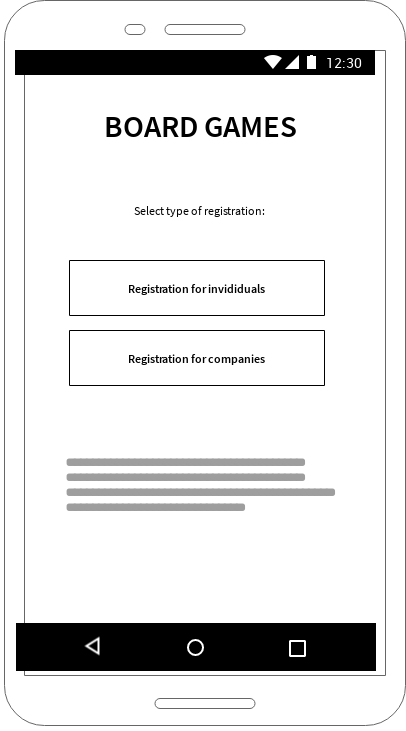
\includegraphics[scale=0.9]{img/entrance_window}
	\label{img:entrance_window}
\end{figure}

\begin{figure}[H]
	\centering
	\caption{Naujos kompanijos registracijos langas}
	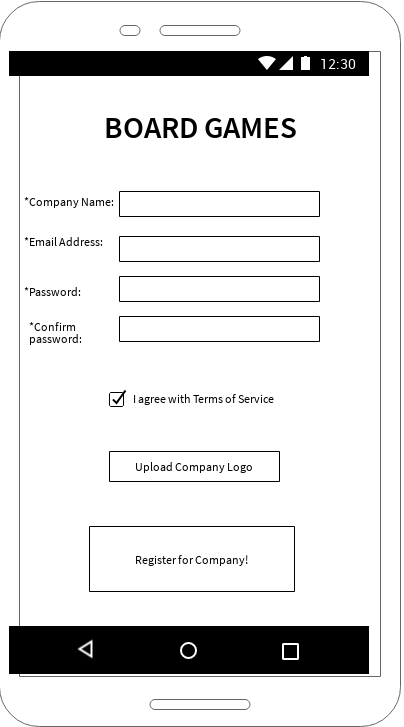
\includegraphics[scale=0.9]{img/company_register}
	\label{img:company_register}
\end{figure}

\begin{figure}[H]
	\centering
	\caption{Prisijungimo langas}
	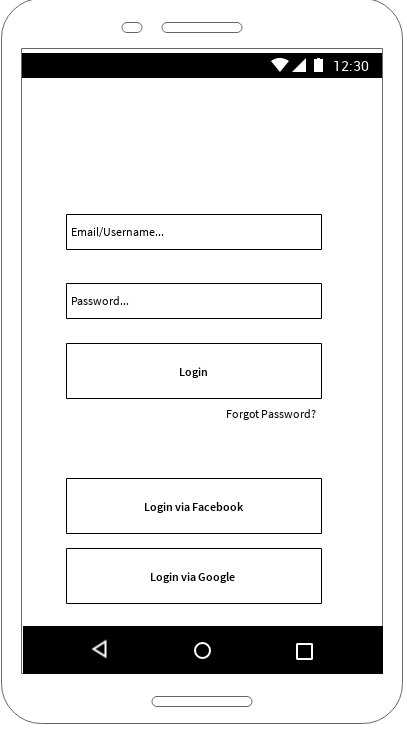
\includegraphics[scale=0.9]{img/login_window}
	\label{img:login_window}
\end{figure}

\begin{figure}[H]
	\centering
	\caption{Pagrindinis langas}
	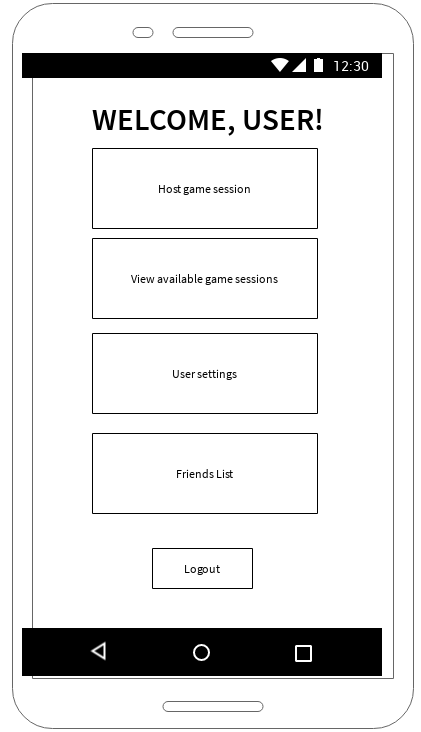
\includegraphics[scale=0.9]{img/main_window}
	\label{img:main_window}
\end{figure}

\begin{figure}[H]
	\centering
	\caption{Žaidimo kūrimo langas}
	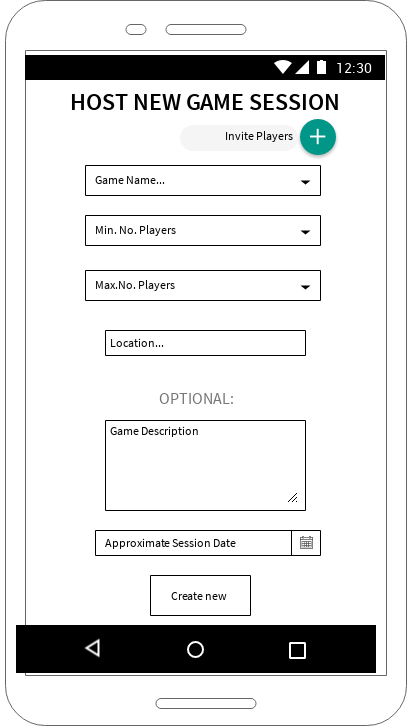
\includegraphics[scale=0.9]{img/host_game_window}
	\label{img:host_game_window}
\end{figure}

\begin{figure}[H]
	\centering
	\caption{Žaidimų pasirinkimo langas}
	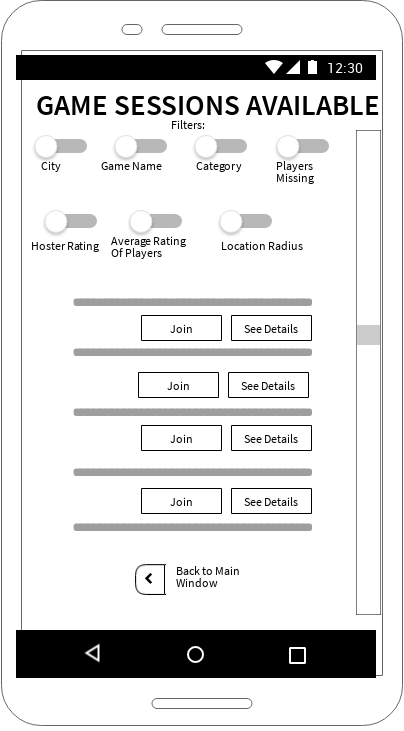
\includegraphics[scale=0.9]{img/game_sessions_view}
	\label{img:game_sessions_view}
\end{figure}

\subsection{Rezultatas}
Dokumente detaliai apibrėžti mobiliosios stalo žaidimų programėlės architektūros funkciniai reikalavimai iš asmeninio vartotojo, kompanijos, administracijos perspektyvos, taip pat nefunkciniai, vartotojo sąsajos reikalavimai. Pagal užsakovo poreikius išskirtos dvi vartotojų kategorijos - paprasti vartotojai, žaidžiantys stalo žaidimus ir stalo žaidimų kūrimo kompanijos, pranešančios naujienas, organizuojančios konkursus, matančios stalo žaidimų sesijų visumos statistiką. Taip pat dokumento priede pateikti numatomos sistemos vartotojo sąsajos brėžiniai, leidžiantys geriau suvokti numatomas sistemos sąsajos galimybes.

\subsection{Išvada}
Apibrėžtų stalo žaidimų programėlės architektūros reikalavimų visuma leidžia vykdyti tolimesnį etapą - konkrečios sistemos kūrimo darbus, pasitelkiant IT architektus ir programuotojus. Sukurtų reikalavimų sėkmės požymis - dokumentas vienareikšmiškai vienodai suvokiamas tiek verslo aplinkos žmonių, tiek ir IT srities atstovų.


\section{4+1 architektūrinis modelis}

\subsection{Fizinis pjūvis}
Šioje dalyje pateikta informacija apie sistemos fizinius mazgus, juose įdiegtas vykdomasias aplinkas, reikalingas vykdyti programos komponentų darbą, taip pat apie komunikaciją tarp mazgų ir juose įdiegtus artifaktus, kurie saugo programinį kodą.
	\subsubsection{Fiziniai mazgai tinkle, jų komunikacija}
				\begin{figure}[H]
				\centering
				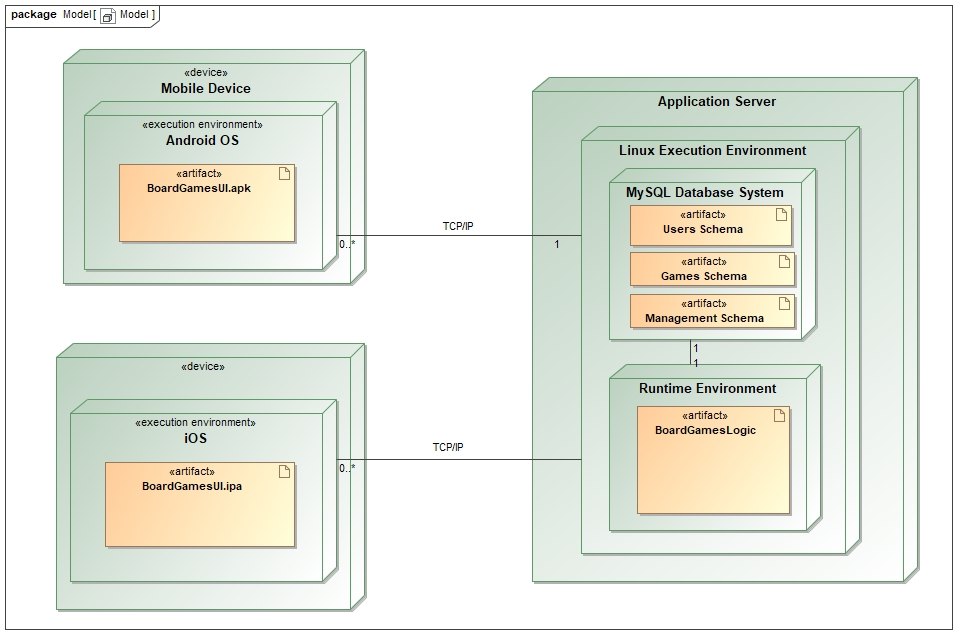
\includegraphics[scale=0.5]{img/NodesCommunication}
				\caption{Fizinių sistemos mazgų išdėstymo tinkle diagrama}
				\label{img:NodesCommunication}
			\end{figure}
			Mobilioji aplikacija dėl savo paprasto loginio pobūdžio nereikalauja 				kompleksiškos tinklo architektūros su daugybe fizinių komponentų. 				Išdėstymo diagramoje (žr. \ref{img:NodesCommunication} pav.)  pateiktas kliento mazgas – mobilusis įrenginys – 				kuriame veikia Android OS arba iOS. Šiose operacinių sistemų aplinkose 				diegiamas mobiliosios aplikacijos artifaktas (.apk – Android atveju, .ipa 				– iOS atveju), kurį sudaro visos sukompiliuotos projekto vartotojo sąsajos 				klasės, resursai, taip pat ir nesukompiliuoti resursai. Kitas mazgas – 				nutolęs aplikacijos serveris, su kuriuo TCP/IP protokolu komunikuoja kliento mobilusis įrenginys. Šiame nutolusiame fiziniame serveryje veikia stabili Linux OS 				aplinkos distribucija, užtikrinanti duombazės pasiekiamumą ir darbo 				nepertraukiamumą. Šioje OS instaliuota MySQL duomenų bazių valdymo 				sistema, kurioje sukurtos trys lentelių schemos: Users (informacija, 				susijusi su aplikacijos naudotojais), Games (informacija, susijusi su 				žaidimais, jų sesijomis), Management (aplikacijos valdymo, statistinių 				duomenų schema). Taip pat šioje Linux aplinkoje veikia programėlės loginio 				kodo vykdomoji aplinka, kurioje įdiegtas loginis artifaktas, atsakingas už 				visą programėlės logiką.
	\subsubsection{Artifaktų diegimas į mazgus}
				\begin{figure}[H]
				\centering
				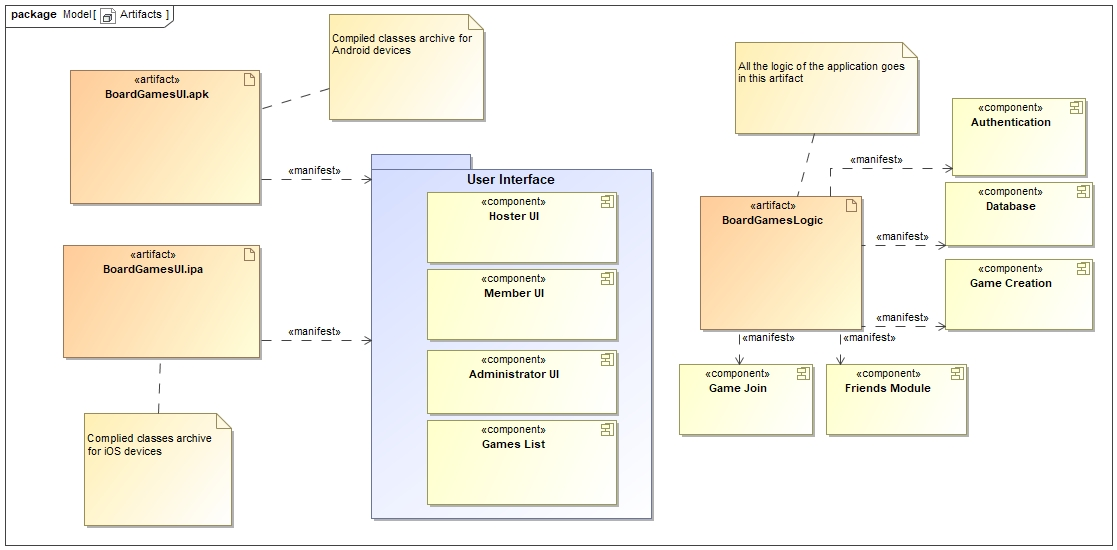
\includegraphics[scale=0.4]{img/Artifacts}
				\caption{Artifaktų sandara ir diegimas į mazgus}
				\label{img:Artifacts}
			\end{figure}
			Sistemą sudaro du pagrindiniai artifaktai - įdiegtas vartotojo sąsajos 				paketas, išdėstomas kliento mobiliajame įrenginyje, ir logikos paketas, 			įdiegtas nutolusio aplikacijos serverio kodo vykdomojoje aplinkoje (žr. \ref{img:Artifacts} pav.) . 
		\subsubsubsection*{Mobiliajame įrenginyje įdiegto artifakto turinys:}
  				\begin{itemize}
					\item Žaidimo šeimininko vartotojo sąsajos komponentas
					\item Paprasto programėlės naudotojo vartotojo sąsajos komponentas.
					\item Administratoriaus vartotojo sąsajos komponentas
					\item Esamų žaidimų sąrašas ir informacija apie juos
				\end{itemize}
		\subsubsubsection*{Nutolusiame serveryje įdiegto artifakto turinys:}
  				\begin{itemize}
					\item Autentifikacijos komponentas - visa logika, susijusi 						su prisijungimu, registracija 
					\item Duombazės komponentas - logika, kurioje apibrėžta 					komunikacija su DBVS
					\item Žaidimo sukūrimo logika - validacija, patvirtinimas, 
					sistemos informavimas
					\item Prisijungimo prie žaidimo logika - validacija, 						žaidimo šeimininko, kitų žaidėjų informavimas 
					\item Draugų modulio komponentas - visa logika, 					apibrėžianti galimą tarpusavio komunikaciją tarp 						programėlės naudotojų
				\end{itemize}
			Taip pat nutolusiame serveryje veikiančios Duomenų bazės valdymo 				sistemos aplinkoje įdiegti šie artifaktai, apibrėžiantys loginį 			duomenų bazės lentelių išskaidymą:
  				\begin{itemize}
					\item Naudotojų lentelių schema
					\item Žaidimų lentelių schema
					\item Valdymo, priežiūros lentelių schema
				\end{itemize}
	\subsubsection{Topologinio išdėstymo tinkle pavyzdys}
				\begin{figure}[H]
				\centering
				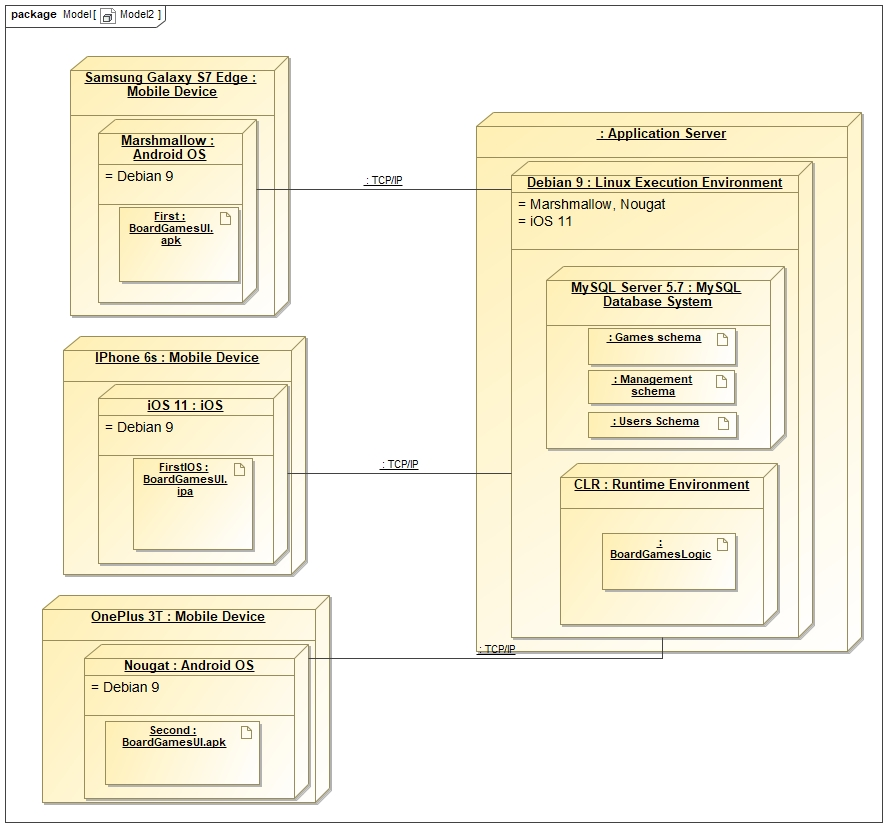
\includegraphics[scale=0.4]{img/TopologyExample}
				\caption{Fizinio išdėstymo tinkle pavyzdys, komunikacija}
				\label{img:TopologyExample}
			\end{figure}
		Diagramoje (žr. \ref{img:TopologyExample} pav.) pavaizduotas galimas realaus sistemos vaizdo atvejis, kuris atitinka 		anksčiau aprašytą mazgų komunikacijos ir artifaktų diegimo logiką. Pavyzdyje 			pateikti trys klientiniai įrenginiai (2 Android, 1 iOS), kurie TCP/IP protokolo 		pagalba komunikuoja su konkrečiu Linux Debian 9.0 distribucijos serveriu, kuriame 			įdiegtas MySQL 5.7 versijos serveris, apdorojantis programėlės SQL užklausas ir 		Common Language Runtime vykdomoji aplinka, apdorojanti loginį programinį kodą, jį 			paverčianti mašininiu, kurį vėliau įvykdo fizinis mazgas.

\subsection{Kūrimo pjūvis}
Komponentų dekompozicija įgyvendinta taip: nuo bendresnių komponentų pereinanama iki detalesnių.

	\subsubsection{Bendroji UML diagrama}
		\begin{figure}[H]
			\centering
			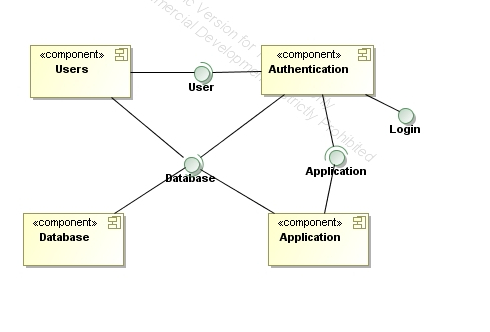
\includegraphics[scale=0.6]{img/UMLComponent1}
			\caption{Bendroji UML diagrama}
			\label{img:UMLComponent1}
		\end{figure}
		Vartotojui įsijungus stalo žaidimų aplikaciją, jis prie jos turi prisijungti, kad būtų patvirtinta jo tapatybė. Tai atliekama prisijungimo sąsajoj, kurią suteikia autentifikacijos komponentas. Patikrinus duomenis duomenų sistemoje, kurioje saugoma informacija apie vartotoją bei jo įvertinimą, gautą iš kitų žaidėjų, ir sėkmingai autentifikavus vartotoją, jam leidžiama naudotis stalo žaidimų aplikacijos ir naudotojo komponentų teikiamomis funkcijomis. Naudotojo komponento teikiama sąsaja leidžia pateikti informaciją apie save kitiems, o aplikacijos komponento sąsaja suteikia galimybę kurti žaidimus, prisijungti prie jų, vertinti vartotojus, pateikti informaciją apie esančius žaidimus pačiam vartotojui ar pačio kuriamus kitiems vartotojams (žr. \ref{img:UMLComponent1} pav.) .
		
		\subsubsection{Vartotojo komponentų diagrama}
		Aukščiau pateikta UML diagrama, kurioje vaizduojami bendri komponentai. Atskirus sistemos komponentus patogiau vaizduoti atskirai, todėl tam sukurtos papildomos diagramos.
		
		\begin{figure}[H]
			\centering
			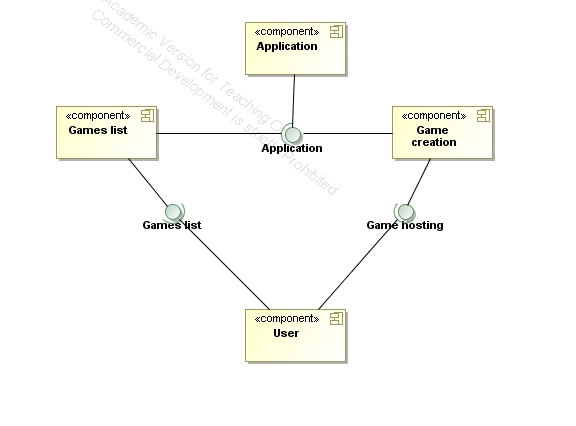
\includegraphics[scale=0.6]{img/UMLComponent2}
			\caption{Vartotojo komponentų diagrama}
			\label{img:UMLComponent2}
		\end{figure}
		Vartotojui pateikiama atitinkama sąsaja priklausomai nuo to, ar vartotojas pasirinko būti žaidimo kūrėju, ar prisijungti prie žaidimo. Jei vartotojas pasirinko prisijungti prie esamo žaidimo, tai jam yra pateikiama žaidimų sąrašo sąsaja, pateikianti sąrašą žaidimų, kuriuose trūksta narių. Jei vartotojas nusprendė pats kurti žaidimą, tada jis nukeliamas į žaidimo kūrimo langą ir įgauna papildomų funkcijų. Tai suteikia žaidimo kūrimo komponentas ir jo suteikiama žaidimo organizavimo sąsaja. Pasirinkimą būti žaidimo kurėju ar paprastu nariu bet kada galima pakeisti(žr. \ref{img:UMLComponent2} pav.) . 
		
		\subsubsection{Detalesnė vartotojo komponentų diagrama}
		Kadangi vartotojai gali arba prisijungti prie žaidimų, arba būti jų kūrėjais, jiems reikalingi atitinkami komponentai. Kad geriau matytųsi, kokie iš jų priklauso kiekvienam tipui, sukurta atskira UML diagrama.
		
		\begin{figure}[H]
			\centering
			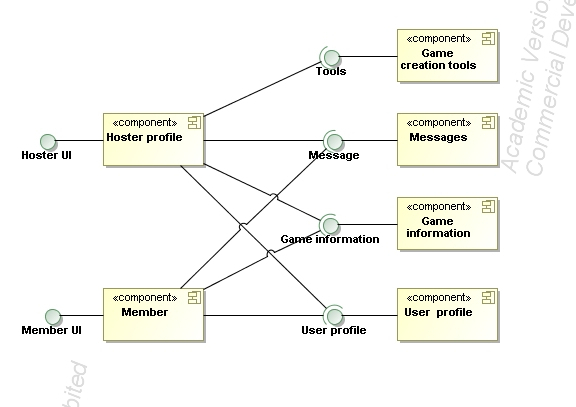
\includegraphics[scale=0.6]{img/UMLComponent3}
			\caption{Detalesnė vartotojo komponentų diagrama}
			\label{img:UMLComponent3}
		\end{figure}
		Tiek paprasti nariai, tiek kūrėjai gali naudotis vartotojo profilio, žaidimo informacijos ir žinučių komponentais, kurie suteikia atitinkamas sąsajas. Vartotojo profilio komponentas leidžia parodyti informaciją apie žaidimuose esančius narius bei jų įvertinimą ir patikimumą. Žaidimo informacijos komponente trumpai nupasakojama apie žaidimą bei pateikiamas jo pavadinimas. Žinučių komponentas suteikia galimybę susisiekti su kiekvienu žaidimo nariu atskirai ir bendrauti bendrame grupės pokalbyje. Kūrėjas taip pat gali naudotis žaidimo kūrimo įrankių komponentu. Jam suteikiamos galimybės pateikti ir keisti žaidimo informaciją, priimti, pakviesti bei išmesti žaidimo narius (žr. \ref{img:UMLComponent3} pav.) .

			
\subsection{Loginis pjūvis}
	\subsubsection{Klasių Diagramos}
			Tam, kad būtų patogiau suprasti, klasių diagrama yra padalinta į kelias dalis:
		\subsubsubsection*{Pirmoji klasių diagramos dalis :}
			\begin{figure}[H]
				\centering
				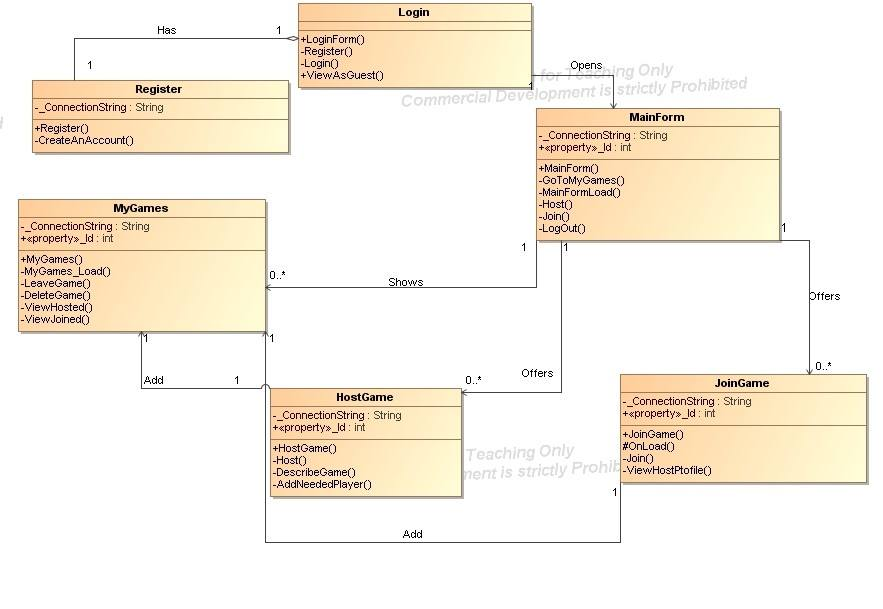
\includegraphics[scale=0.5]{img/BoardGamesClassDiagram}
				\caption{Klasių diagrama: registracija ir pgr funkcijos}
				\label{img:BoardGamesClassDiagram}
			\end{figure}
			Klasė Login, atsakinga už vartotojo autentifikaciją, turi  registracjos langą (klasę Register) (žr. \ref{img:BoardGamesClassDiagram} pav.) . Viena Login klasė gali turėti vieną   registracijos klasę. Užsiregistravus, Login klasė gali atidaryti pagrindinį vartotojo puslapį (MainForm klasę), kuris gali parodyti MyGames klasę, t.y. vartotojo žaidimus , siūlo sukurti žaidimą (HostGame) arba jungtis prie jau egzistuojančio (JoinGame) žaidimo. Kiekviena MainForm klasė gali parodyti, sukurti ir prisijungti prie kiek norimai daug žaidimų. Kiekvieną kartą sukūrus ar prisijungus prie žaidimo, jis yra pridedamas prie MyGames. 
		\subsubsubsection*{Antroji klasių diagramos dalis :}
			\begin{figure}[H]
				\centering
				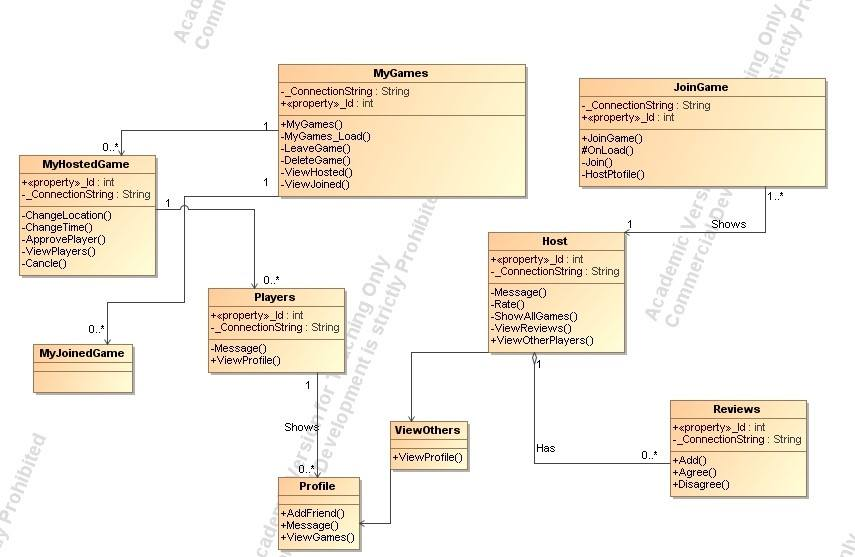
\includegraphics[scale=0.5]{img/BoardGamesClassDiagrampt1}
				\caption{Klasių diagrama: žaidimų kūrimas ir prisijungimas}
				\label{img:BoardGamesClassDiagrampt1}
			\end{figure}
			Klasė MyGames atveria vartotojo sukurtus žaidimus (klasė MyHostedGame) bei žaidimus, prie kurių jis prisijungė (MyJoinedGame) (žr. \ref{img:BoardGamesClassDiagrampt1} pav.) . Abiejų variantų vartotojas gali turėti kiek norimai daug. Kiekvienas sukurtas žaidimas gali atverti prisijungusių kitų žaidėjų sąrašą ir iš jo yra pasiekiamas kiekvieno žaidėjo profilis (klasė Profile). Jei vartotojas pasirinko prisijungti prie žaidimo, už tai yra atsakinga JoinGame klasė, kurios vieną ar daugiau elementų (žaidimų) sukūrė konkretus kūrėjas (klasė Host). Host turi klasę Reviews, nes kiekvienas kūrėjas gali turėti atsiliepimų. Prisijungus prie žaidimo, klasė ViewOthers užtikrina galimybę peržvelgti kitų prisijungusių žaidėjų sąrašą ir jų profilius (Profile).
		\subsubsubsection*{Trečioji klasių diagramos dalis :}
			\begin{figure}[H]
				\centering
				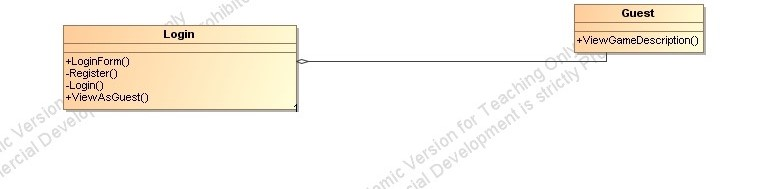
\includegraphics[scale=0.5]{img/BoardGamesClassDiagrampt2}
				\caption{Klasių diagrama: Svečias}
				\label{img:BoardGamesClassDiagrampt2}
			\end{figure}
			Jei vartotojas nėra prisiregistravęs (Guest), Login forma gali nuvesti jį prie sukurtų žaidimų sąrašo (žr. \ref{img:BoardGamesClassDiagrampt2} pav.) .
		\subsubsubsection*{Pilna klasių diagrama :}
			\begin{figure}[H]
				\centering
				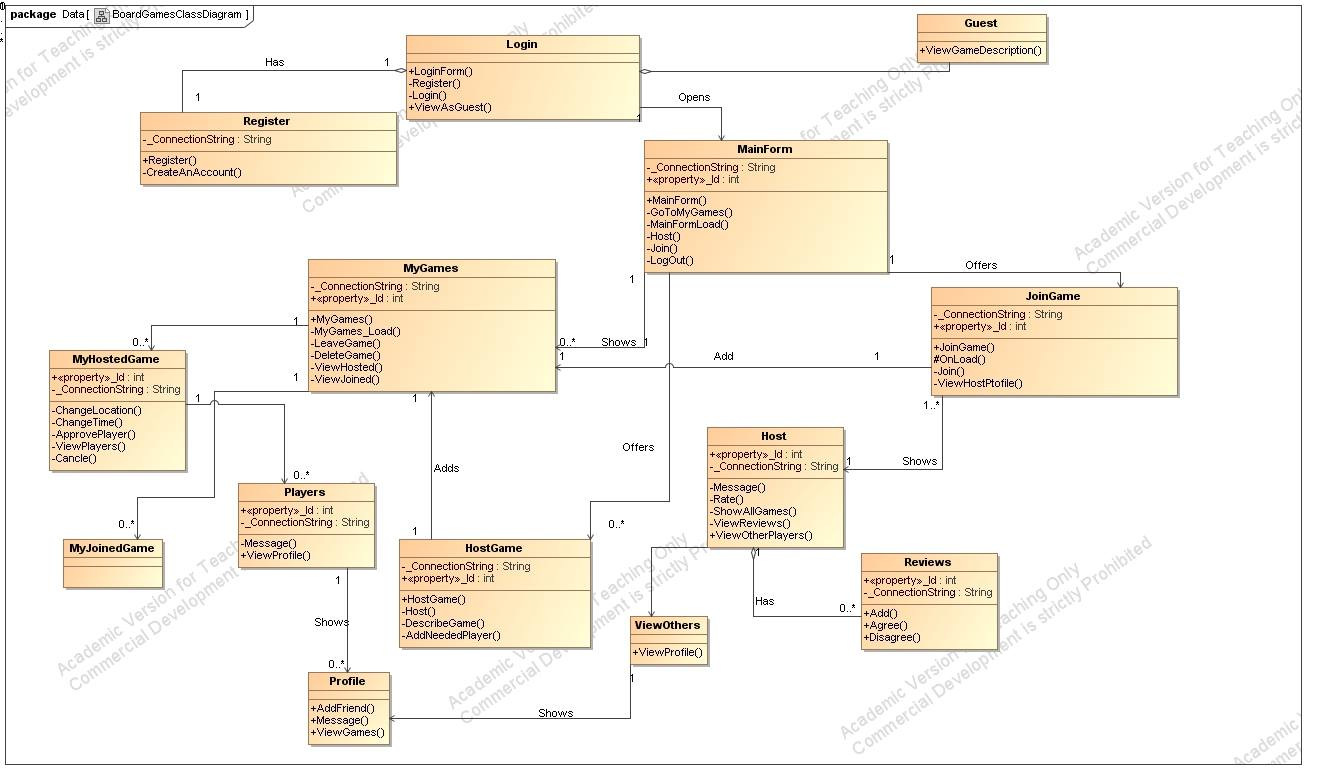
\includegraphics[scale=0.4]{img/BoardGamesClassDiagramFull}
				\caption{Visa klasių diagrama}
				\label{img:BoardGamesClassDiagramFull}
			\end{figure}
	\subsubsection{Objektų diagrama}
		\begin{figure}[H]
				\centering
				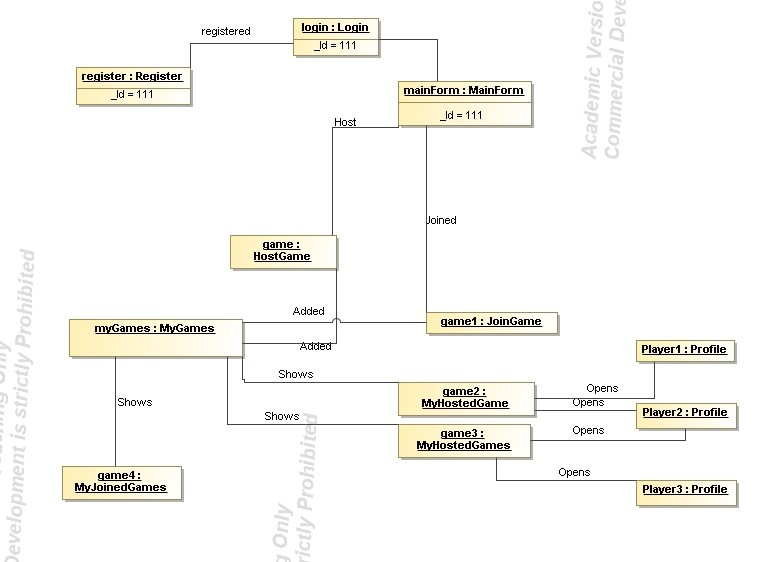
\includegraphics[scale=0.5]{img/Object}
				\caption{Objektų diagrama}
				\label{img:Object}
			\end{figure}
		Užsiregistravęs vartotojas yra autentifikuojamas ir nusiunčiamas į savo pagrindinį puslapį mainForm (žr. \ref{img:Object} pav.) . Jis buvo sukūręs žaidimą game ir prisijungęs prie žaidimo game1, kurie abu buvo pridėti prie jo asmeninių žaidimų sarašo myGames. Jame jau yra žaidimai game2 ir game3 (kuriuos jis sukūrė pats) bei game4, prie kurio buvo prisijungęs. Kitas vartotojas player1 buvo prisijungęs prie žaidimo game2, player2 - prie game2 ir game3, o player3 - prie game3.

\subsection{Užduotys}
Pagrindinės sistemos užduotys ir su jomis susiję agentai

	\renewcommand{\labelitemi}{$\bullet$}
	\renewcommand{\labelitemii}{$\circ$}
	\begin{itemize}
		\item Agentai:
			\begin{description}
				\item [$\circ$ Svečias] Neprisijungęs programėlės naudotojas.
				\item [$\circ$ Registruotas vartotojas] Žmogus, sėkmingai atlikęs registraciją ir prisijungęs prie programėlės, galintis dalyvauti jos veikloje.
				\item [$\circ$ Žaidimo dalyvis] Registruotas vartotojas, nusprendęs prisijungti prie vieno iš sistemos siūlomų žaidimų.
				\item [$\circ$ Žaidimo šeimininkas] Registruotas vartotojas, pridėjęs žaidimą sistemoje.
				\item [$\circ$ Administratorius] Žmogus, atsakingas už tinkamą sistemos darbo palaikymą.
			\end{description}
	\end{itemize}
		
	\subsubsubsection*{Pagrindinės užduotys}
	
	\subsubsection{Svečio ir registruoto vartotojo užduotys}
		\begin{figure}[H]
			\centering
			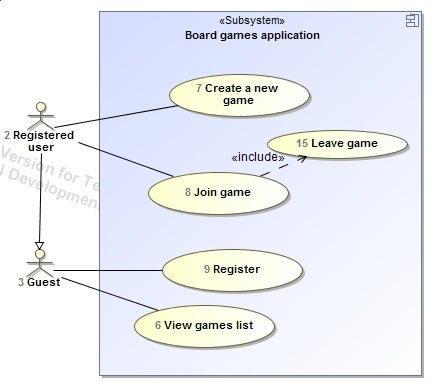
\includegraphics[scale=0.6]{img/UzduociuDiagrama1}
			\caption{Svečio ir registruoto vartotojo užduotys}
			\label{img:UzduociuDiagrama1}
		\end{figure}
		Kol vartotojas nėra užsiregistravęs sistemoje, jam suteikiamos svečio teisės, kurios leidžia tik peržiūrėti sukurtus žaidimus. Norėdamas įgyti daugiau privilegijų, vartotojas privalo užsiregistruoti. Registruotas vartotojas jau gali dalyvauti programėlės veikloje: sukurti naują žaidimą ir apie jį paskelbti, arba prisijungti prie jau esamo (žr. \ref{img:UzduociuDiagrama1} pav.) .

	\subsubsection{Žaidimo dalyvio ir šeimininko užduotys}
		\begin{figure}[H]
			\centering
			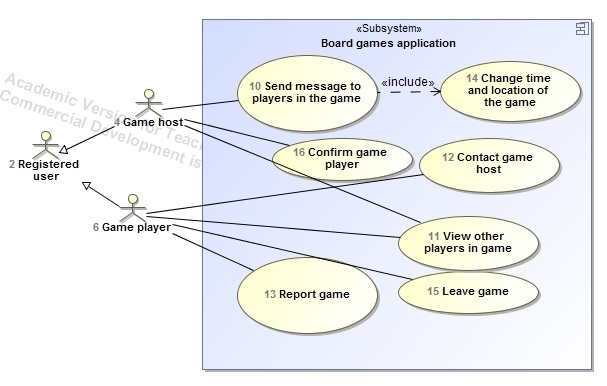
\includegraphics[scale=0.5]{img/UzduociuDiagrama2}
			\caption{Žaidimo dalyvio ir šeimininko užduotys}
			\label{img:UzduociuDiagrama2}
		\end{figure}
		Registruotas vartotojas gali atlikti du vaidmenis: arba būti sukurto žaidimo šeimininku, arba paprasčiausiu dalyviu (žr. \ref{img:UzduociuDiagrama2} pav.) . Žaidimo dalyviui leidžiama pranešti sistemos administratoriui apie nevykstantį žaidimą, tuo atveju, jeigu žaidėjas nuvyko į sutartą žaidimo vietą reikiamu laiku ir jam nepavyko surasti kitų užsiregistravusių dalyvių. Jeigu bent vienas žaidėjas (išskyrus šeimininką) nesutinka su tokia informacija, pranešimas laikomas melagingu. Priešingu atveju, sulaukus administratoriaus pritarimo, žaidimas išimamas iš aktyvių žaidimų sąrašo norint užkirsti tolimesnį galimą dalyvių pritraukimą. Tai pat, šeimininkui patvirtinus žaidėją, jis įgauna teisę peržiūrėti kitų, jau pareiškusių norą dalyvauti žaidėjų profilius ir su jais susipažinti naudojantis programėlės asmeninių žinučių sistema. Norėdamas pasiteirauti dėl žaidimo detalių arba visais kitais iškilusiais klausimais, jis taip pat gali tiesiogiai kreiptis į žaidimo šeimininką. Šeimininkas gali informuoti žaidėjus apie nenumatytai pasikeitusią žaidimo vietą ar laiką, susisiekti su jais ir iš anksto trumpai supažindinti su žaidimo taisyklėmis. Jeigu žaidimo dalyviui nepatinka kitų dalyvių kompanija ar bet kokios kitos žaidimo detalės, jis gali bet kada palikti žaidimą, o žaidimo šeimininkas apie tai yra informuojamas.

	\subsubsection{Sistemos administravimas}
		\begin{figure}[H]
			\centering
			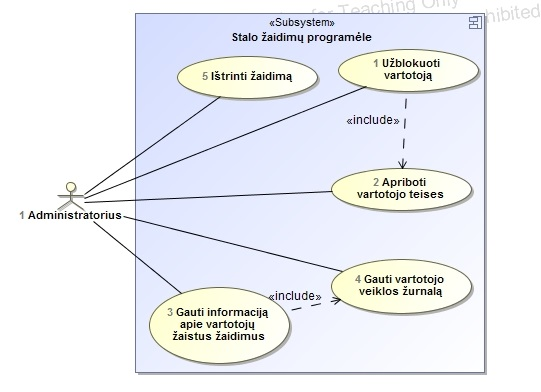
\includegraphics[scale=0.6]{img/UzduociuDiagrama3}
			\caption{Sistemos administravimas}
			\label{img:UzduociuDiagrama3}
		\end{figure}
		Administratorius prižiūri programėlės pateikiamos informacijos patikimumą (žr. \ref{img:UzduociuDiagrama3} pav.) . Jis turi teisę ištrinti registruoto vartotojo sukurtą žaidimą siekdamas apsaugoti dar vėliau prie žaidimo galimai prisijungsiančius dalyvius tuo atveju, jei vartotojo pateikti duomenys nėra tikslūs ar apie žaidimą jau buvo gautas įspėjamas pranešimas iš kitų sąžiningų vartotojų. Jeigu vartotojas nesiliauja kurti fiktyvių žaidimų, jam gali būti taikomos nuobaudos: laikinai (pvz. parai) apribojimas organizuoti bet kokius žaidimus. Jei tai kartojasi, administratorius gali apsvarstyti pasiūlymą užblokuoti vartotojo paskyrą ir įtraukti jį į nepageidaujamų sąrašą. Kaip pagalbinę priemonę vartotojų veiksmams sekti administratorius gali naudoti vartotojų veiklos žurnalą, kuriame būtų pateikiami chronologiškai surikiuoti vartotojų veiksmai, gauti nurodžius dominantį periodą. Veiklos žurnalą būtų galima filtruoti pagal konkretų vartotoją, taip susiaurinant paiešką.		


\subsection{Procesų pjūvis}
Aplikacijoje yra vartotojo sąsajos, duomenų apdorojimo ir duomenu bazės procesai. 
Vartotojas tiesiogiai bendraudamas su vartotojo sąsaja, siunčia asinchronines 
žinutes duomenų apdorojimo procesui, kuris savo ruožtu bendrauja su duomenų baze.

	\subsubsection{Prisijungimas}
		\subsubsubsection*{Prisijungimo procesų sekos diagrama :}
		\begin{figure}[H]
			\centering
			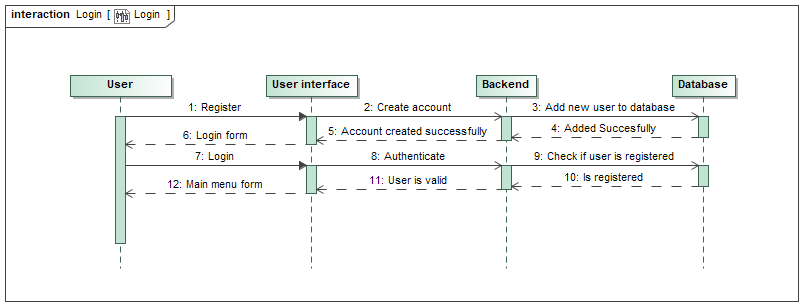
\includegraphics[scale=0.5]{img/Login_sequence}
			\caption{Prisijungimo procesų sekų diagrama}
			\label{img:Login_sequence}
		\end{figure}
		Visų pirma vartotojas privalo užsiregistruoti. Vartojo sąsaja nusiunčia JSON 
		žinutę su gautais duomenimis loginiam procesui, kuris patikrina ar duomenys yra tinkami ir
		prideda vartotoją į duomenų bazę. Užsiregistravęs vartotojas turi prisijungti,
		procedūra ganėtinai panaši - vartotojo sąsajoje gauti duomenys patikrinami ir 
		jei jie yra validūs, patikrinama ar slaptažodis sutampa su esančiu duomenų
		bazėje. Autentifikuotas vartotojas yra prijungiamas prie programėlės. 
		Jei slaptažodis netinka arba vartotojas nerastas duomenų bazėje, leidžiama
		patikslinti prisijungimo laukus ir prisijungimo procesas kartojamas dar kartą (žr. \ref{img:Login_sequence} pav.).
		\subsubsubsection*{Prisijungimo/Registracijos procesų veiklos diagrama :}
		\begin{figure}[H]
			\centering
			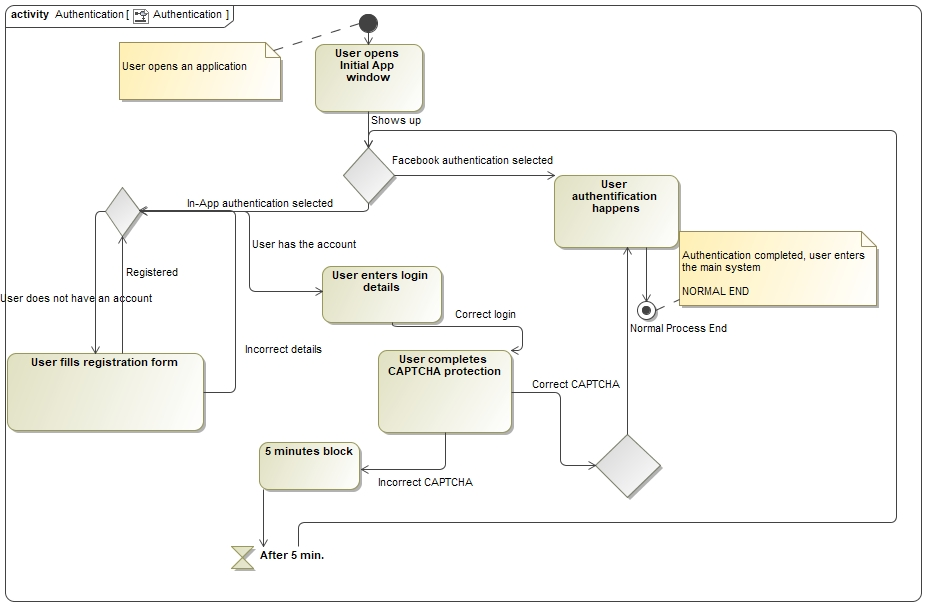
\includegraphics[scale=0.5]{img/Authentication}
			\caption{Autentifikacijos veiklos diagrama}
			\label{img:Authentication}
		\end{figure}
		Kiekvienas programėlės naudotojas patenka į prisijungimo langą, kuriame gali 			pasirinkti vieną iš galimų prisijungimo būdų - naudojantis Facebook API arba 			paprasta vartotojo paskyra (žr. \ref{img:Authentication} pav.). Pasirinkus Facebook autentifikacija, programėlė 			nuskaito vartotojo identifikacinius duomenis ir ši veikla pabaigiama. Pasirinkus 			prisijungimą naudojantis paprasta paskyra atsiranda dvi galimybės - prisijungti 		arba užsiregistruoti. Pasirinkus registraciją vartotojas suveda savo duomenis, 			jeigu pastarieji teisingi - jis užregistruojamas ir gali prisijungti. Jei duomenys 			klaidingi - vartotojas vėl patenka į tą patį registracijos langą. Norėdamas 			prisijungti vartotojas turi įvesti savo teisingus prisijungimo duomenis, tuomet 		iššoka CAPTCHA patvirtinimo paveikslėlis, skirtas prevencijai nuo kenkėjiško tipo 			skriptų ir programų, imituojančių žmogų. Jeigu CAPTCHA klaidingas - vartotojas 			blokuojamas 5 minutėms (tiek laiko negali prisijungti siekiant taupyti sistemos 		resursus, išvengti DOS/DDOS atakų). Suvedus teisingą CAPTCHA kodą patenkama į 			sistemą ir ši veikla užbaigiama.
	\subsubsection{Pagrindinis navigacijos langas}
		\subsubsubsection*{Vartotojo perspektyva :}
			\begin{figure}[H]
				\centering
				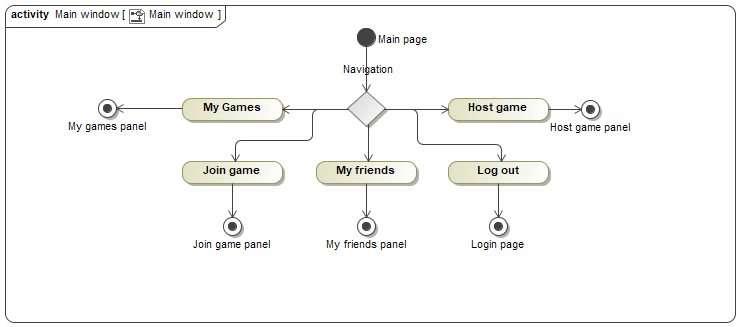
\includegraphics[scale=0.5]{img/MainWindow_activity}
				\caption{Pagrindinio navigacijos lango veiklos diagrama iš vartotojo perspektyvos}
				\label{img:MainWindow_activity}
			\end{figure}
			\subsubsubsection*{Pagrindiniame navigacijos lange vartotojas paspaudęs atitinkamus mygtukus (žr. \ref{img:MainWindow_activity} pav.) gali:}
				\renewcommand{\labelitemi}{$\bullet$}
				\begin{itemize}
					\item Atidaryti žaidimo sukūrimo langą.
					\item Atidaryti prisijungimo prie žaidimo langą.
					\item Atidaryti draugų sąrašo langą.
					\item Atidaryti mano žaidimų langą
					\item Atsijungti
				\end{itemize}
				
		\subsubsubsection*{Administratoriaus perspektyva :}
			\begin{figure}[H]
				\centering
				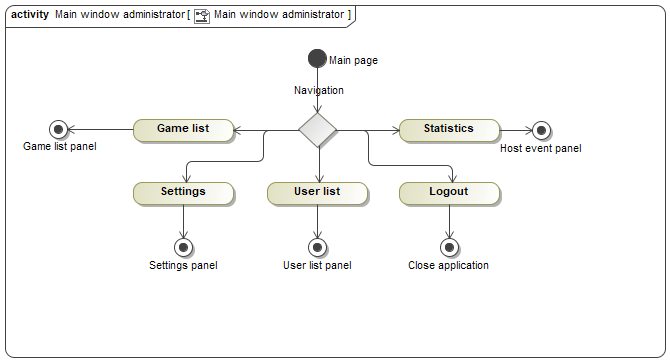
\includegraphics[scale=0.5]{img/MainWindowAdministrator}
				\caption{Pagrindinio navigacijos lango veiklos diagrama iš administratoriaus perspektyvos}
				\label{img:MainWindowAdministrator}
			\end{figure}
			\subsubsection*{Pagrindiniame navigacijos lange vartotojas paspaudęs atitinkamus mygtukus (žr. \ref{img:MainWindowAdministrator} pav.) gali:}
				\renewcommand{\labelitemi}{$\bullet$}
				\begin{itemize}
					\item Atidaryti visų žaidimų sąrašą.
					\item Atidaryti profilio nustatymo langą.
					\item Atidaryti visų vartotojų sąrašą.
					\item Atidaryti statistikos langą
					\item Atsijungti
				\end{itemize}
				
		\subsubsubsection*{Kompanijos perspektyva :}
			\begin{figure}[H]
				\centering
				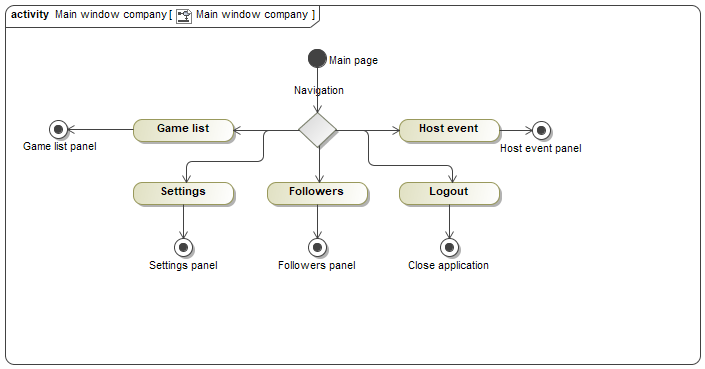
\includegraphics[scale=0.5]{img/MainWindowCompany}
				\caption{Pagrindinio navigacijos lango veiklos diagrama iš kompanijos perspektyvos}
				\label{img:MainWindowCompany}
			\end{figure}
			\subsubsubsection*{Pagrindiniame navigacijos lange vartotojas paspaudęs atitinkamus mygtukus (žr. \ref{img:MainWindowCompany} pav.) gali:}
				\renewcommand{\labelitemi}{$\bullet$}
				\begin{itemize}
					\item Atidaryti savo sukurtų žaidimų sąrašą.
					\item Atidaryti profilio nustatymo langą.
					\item Atidaryti sekėjų sąrašą.
					\item Atidaryti renginio sukūrimo langą
					\item Atsijungti
				\end{itemize}

	\subsubsection{Žaidimo sukūrimo langas}
		\subsubsubsection*{Žaidimo sukūrimo veiklos diagrama :}
			\begin{figure}[H]
				\centering
				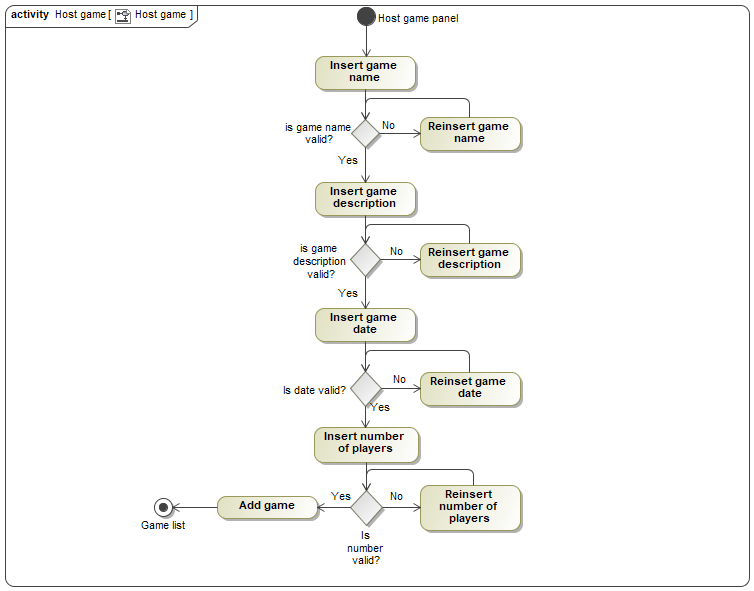
\includegraphics[scale=0.5]{img/HostGame_activity}
				\caption{Žaidimo sukūrimo veiklos diagrama}
				\label{img:Hostgame_activity}
			\end{figure}
			\subsubsubsection*{Žaidimo sukūrimo lange (žr. \ref{img:Hostgame_activity} pav.) vartotojas turi įvesti :}
				\renewcommand{\labelitemi}{$\bullet$}
				\begin{itemize}
					\item Žaidimo pavadinimą.
					\item Žaidimo aprašymą.
					\item Žaidimo datą.
					\item Žaidėjų skaičių
				\end{itemize}
			Įvedimo metu tikrinama ar duomenys įvesti leistinu formatu. Jei formatas 
			netinkamas, vartotojas turi pataisyti atitinkamus duomenų laukus. Tinkamai
			užpildžius laukus,leidžiama pridėti žaidimą.
		\subsubsubsection*{Žaidimo sukūrimo procesų sekų diagrama :}
			\begin{figure}[H]
				\centering
				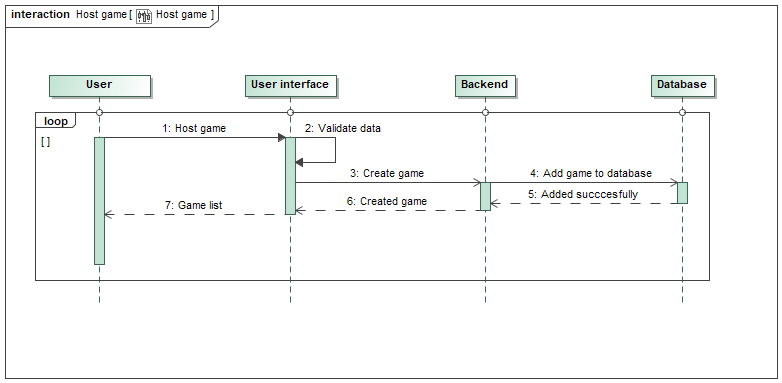
\includegraphics[scale=0.5]{img/HostGame_sequence}
				\caption{Žaidimo sukūrimo procesų sekų diagrama}
				\label{img:Hostgame_sequence}
			\end{figure}
			Vartotojas norėdamas sukurti žaidimą įveda žaidimo duomenis (žr. \ref{img:Hostgame_sequence} pav.). Įvedimo metu 
			tikrinama ar duomenys įvesti leistinu formatu. Jei duomenys tinkami, tada 
			jie JSON formatu išsiunčiami loginiam procesui, kuris sukuria žaidimą ir 
			įrašo jį į duomenų bazę.	
			
	\subsubsection{Prisijungimo prie egzistuojančio žaidimo langas}	
		\subsubsubsection*{Prisijungimo prie egzistuojančio žaidimo veiklos diagrama :}
			\begin{figure}[H]
				\centering
				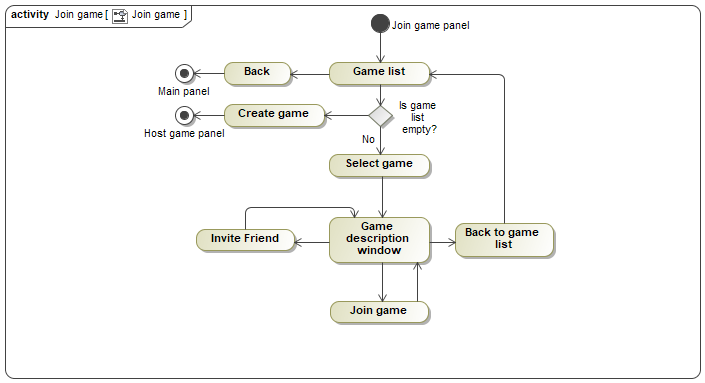
\includegraphics[scale=0.5]{img/JoinGame_activity}
				\caption{Prisijungimo prie egzistuojančio žaidimo veiklos diagrama}
				\label{img:JoinGame_activity}
			\end{figure}
			Iš pradžių vartotojui atidaromas egzistuojančių žaidimų sąrašas (žr. \ref{img:JoinGame_activity} pav.). Čia 
			vartotojas gali grįžti pagrindinį navigacijos langą arba tęsti žaidimo
			pasirinkimą. Jei nėra žaidimų prie kurių būtų galima prisijungti, vartotojui
			pasiūloma sukurti naują žaidimą. Vartotojui sutikus jis nukreipiamas į 
			žaidimo sukūrimo langą. Jei žaidimų sąrašas nėra tučias, tai vartotojas
			gali pasirinkti žaidimą prie kurio norėtų prisijungti. Pasirinkus atidaromas
			pasirinkto žaidimo aprašymo langas. Čia vartotojas gali pakviesti draugus
			kartu žaisti pasirinktą žaidimą, pats prisijungti prie žaidimo arba grįžti
			atgal į žaidimų sąrašą ir pasirinkti kitą žaidimą.
		\subsubsubsection*{Prisijungimo prie egzistuojančio žaidimo sekų diagrama :}
			\begin{figure}[H]
				\centering
				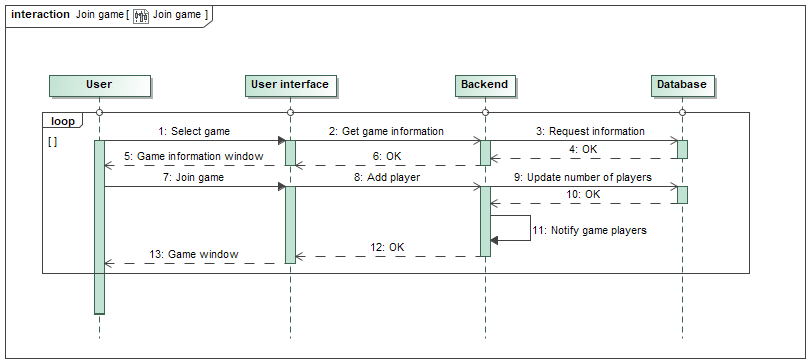
\includegraphics[scale=0.5]{img/JoinGame_sequence}
				\caption{Prisijungimo prie egzistuojančio žaidimo procesų sekų diagrama}
				\label{img:JoinGame_sequence}
			\end{figure}
			Žaidėjui pasirinkus žaidimą iš sąrašo, atidaromas žaidimo informacijos 
			langas (žr. \ref{img:JoinGame_sequence} pav.). Informaciją apie žaidimą suteikia logikos procesas, kuris
			nusiuntęs užklausą į duomenų bazę, gauna papildomą informaciją apie 
			pasirinktą žaidimą. Vartotojui nusprendus prisijungti prie žaidimo, 
			nusiunčiama žinutė atnaujinti prisijungusių žaidėjų skaičių duomenų bazėje,
			taip pat visiems tame žaidime užsiregistravusiems žaidėjams išsiunčiamas 
			pranešimas apie naują prisijungusį žaidėją.

	\subsubsection{Draugų sąrašo langas}		
		\subsubsubsection*{Draugų sarašo lango sekų diagrama :}
			\begin{figure}[H]
				\centering
				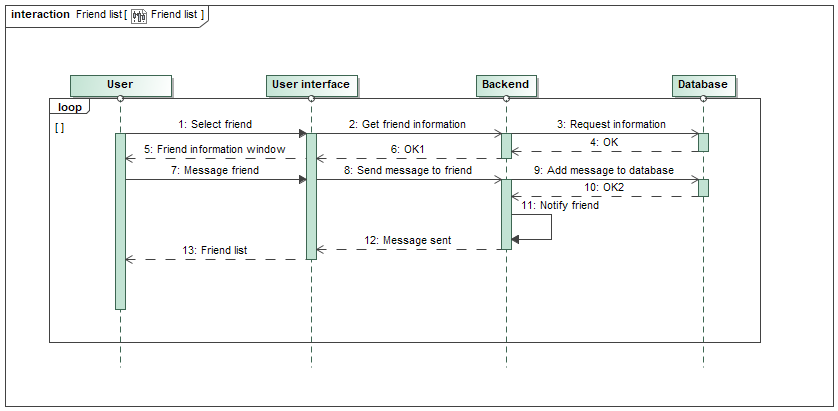
\includegraphics[scale=0.5]{img/FriendList_sequence}
				\caption{Draugų sarašo lango sekų diagrama}
				\label{img:FriendList_sequence}
			\end{figure}
			Vartotojui pasirinkus draugą iš draugų sąrašo, paprašoma loginio proceso
			gauti daugiau duomenų apie draugą iš duomenų bazės (žr. \ref{img:FriendList_sequence} pav.). Tuomet atidaromas 
			langas su daugiau duomenų apie draugą. Paspaudus siųsti žinutę logikos 
			procesas išsaugo žinutę duomenų bazėje ir praneša draugui apie gautą žinutę.
			
	\subsubsection{Žaidimo langas}		
		\subsubsubsection*{Žaidimo lango sekų diagrama :}
			\begin{figure}[H]
				\centering
				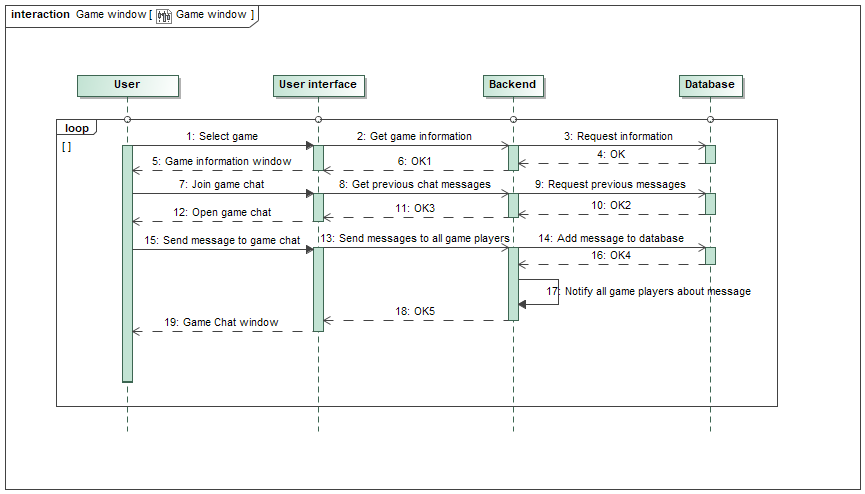
\includegraphics[scale=0.5]{img/GameWindow_sequence}
				\caption{Žaidimo lango sekų diagrama}
				\label{img:GameWindow_sequence}
			\end{figure}
			Vartotojui pasirinkus žaidimą iš žaidimų sąrašo, paprašoma loginio proceso
			gauti daugiau duomenų apie žaidimą iš duomenų bazės (žr. \ref{img:GameWindow_sequence} pav.). Tuomet atidaromas 
			langas su daugiau duomenų apie žaidimą. Paspaudus siųsti žinutę logikos 
			procesas paprašo žaidimo susirašinėjimo istorijos iš duomenų bazės. Tada
			atidaromas pokalbių langas, kur vartotojas gali išsiųsti žinutę visiems 
			prie žaidimo prisijungusiems žaidėjams. Paspaudus siųsti žinutę logikos 
			procesas išsaugo žinutę duomenų bazėje ir praneša žaidėjams apie gautą žinutę.
			
\subsection{Rezultatai}
Šioje dalyje pristatyta mobiliosios stalo žaidimų programėlės Board Games 4+1 architektūra ir
modelis, kurį sudaro loginis, kūrimo, fizinis, procesų ir užduočių pjūviai, atskleidžiantys detalų
ir konkretų projektuojamos sistemos vaizdą.

\sectionnonum{Išvada}
Visos trys projekto dalys, atliktos Programų sistemų inžinerijos kurso metu, leido geriau susipažinti
su vientisu ir nuosekliu IT projekto kūrimo procesu, pradedant nuo detalios verslo srities analizės,
į kurią įeina ir rinkos tyrimai, tęsiant reikalavimų specifikacija, kuri nusako aiškius numatomos
sistemos rėmus ir baigiant aiškiu ir detaliu architektūriniu vaizdu, kurį apibrėžia skirtingi sistemos
architektūriniai pjūviai. Nuoseklus projekto kūrimo procesas, kurio pagal šio kurso turinį buvo bandoma
laikytis, leidžia išvengti netikėtumų eigoje, papildomų nenumatytų kaštų, tobulinimo kliūčių ir labai
tikėtina - greitos sistemos ,,žūties''.
	
\sectionnonum{Literatūros sąrašas}
\begin{itemize}
	\item Doc. dr. K. Petrausko Programų Sistemų Inžinerijos kurso konspektai
    \item A. Abran, J. W. Moore, P.Bourque, R. Dupuis, L. L. Tripp - ,,Guide to the Software Engineering Body of Knowledge''
	\item UML dokumentacija \url{https://www.tutorialspoint.com/uml/uml_2_overview.htm}
	\item OMG UML v.2.5 Dokumentacija diagramoms, žymėjimui
	\item Informacija apie išdėstymo tinkle (Deployment) diagramas, pavyzdžiai \url{http://www.uml-diagrams.org/deployment-diagrams-overview.html} 
	\item https://osp.stat.gov.lt/statistiniu-rodikliu-analize?theme=all\#/
	\item https://www.androidauthority.com/publishing-first-app-play-store-need-know-383572/
	\item https://www.serveriai.lt/
	\item https://www.ovh.com/us/dedicated-servers/
	\item https://adwords.google.com/ko/KeywordPlanner/
	\item https://www.webpagefx.com/SEO-Pricing.html
\end{itemize}

		
\end{document}
